% LaTeX/AMS-LaTeX

\RequirePackage{fix-cm}
%
%\documentclass{svjour3}                     % onecolumn (standard format)
%\documentclass[smallcondensed]{svjour3}     % onecolumn (ditto)
%\documentclass[smallextended]{svjour3}       % onecolumn (second format)
\documentclass[twocolumn]{svjour3}          % twocolumn

%\documentclass{article}

\usepackage{amssymb}
\usepackage{amsmath}
%\usepackage[dvips]{graphicx}
\usepackage{graphicx}
%\usepackage{subcaption}
\usepackage{algorithm}
\usepackage{algorithmic}
\usepackage{cite}
%%%%%%%%%% NEW COMMANDS
\newcommand{\vect}[1]{\boldsymbol{#1}}

%%%%%%%%%% 
\begin{document}

\title{Studying the performance and accuracy of PFEM-2 in the solution of biomedical benchmarks}
\author{Facundo Del Pin\and Chien-Jung Huang\and I\~naki \c{C}aldichoury\and Rodrigo R. Paz}
\institute{Livermore Software Technology Corporation\\ Livermore,  CA, United
States\\
\email{fdelpin@lstc.com}\\
\email{cjhuang@lstc.com}\\
\email{inaki@lstc.com}\\
\email{rpaz@lstc.com}}
\date{\today}

\maketitle

\begin{abstract}
In recent years the biomedical industry has shown increased interest in using numerical methods to assist in the R\&D of medical devices. The long term goal is to reduce the costly and lengthy process that clinical trials take to for the Food and Drug Administration (FDA) to approve a device. For this both FDA and academia are working together to creat laboratory experiment that will help the industry gain confidence in numerical techniques as well as provide software developers with insights on the deficiencies that numerical softeware may have. In this article three bechmarks proposed by the FDA are used to compare experimental results with those of the Finite element method (FEM) and Particle Finite Element Method 2 (PFEM-2). The first benchmark problem is the flow in a nozzle
containing a gradual and sudden change of the diameter. Several flow regimes are studied. The second problem studies the flow in a simplified centrifugal
blood pump under various pump operation conditions. Finally the third benchamrk studies the steady flow in a patient-averaged inferior vena cava. PFEM-2 is regarded as tool with great potential mainly because no stabilization is needed for the Galerkin approximation of the advection term in the transport equations. This could be a big advantage in problems with large gradients as it is the case for flows at high Reynolds number. This paper is an effort to test PFEM-2 in real world engineering applications.

\keywords{Particle Method \and Finite Element \and Biomedical Devices \and CFD \and Benchmarks \and FDA}
\end{abstract}


\section{Introduction}
A key step in the development of medical devices is the testing phase. Regulatory agencies like the Food and Drug Administration require extensive laboratory testing and a long, tedious and expensive clinical trial process before a device is approved for clinical use. In an effort to optimize this process, the industry and the regulatory agencies are looking at numerical methods as an additional tool that could potentially reduce the time of product development, animal testing and cost. A first critical step to do this end is to increase the confidence, reliability and robustness of numerical techniques. The FDA is actively working on this subject by designing laboratory experiments that could be used to evaluate the solution accuracy provided by computational methods launching the Critical Path Initiative (CPI) \cite{cpi} program. The aim of the program is to standardize the use of computational simulation on the design of the blood-contacting medical
devices and analysis of the ratio of hemolysis in them. The goal of this project is to establish the guidelines for
applying Computational Fluid Dynamics (CFD) techniques on the evaluation and the optimization of the medical devices. FDA has proposed two benchmark
problems \cite{cpi1} for CFD verification and validation. The first benchmark problem is the flow in a nozzle
containing a gradual and sudden change of the diameter. The flows at different flow rates which
correspond to different flow regimes are examined. The second study is the flow in a simplified centrifugal
blood pump. The flow field under various pump operation conditions are analyzed. For each benchmark
problem, the experimental results \cite{fda_res,fda_nozzle,fda_pump} and the flow field predicted with numerical simulations \cite{fda_numrob,hariharan_nozzle,nassau_pump,heck_hemo} from
different institutes are collected. The comparison between results obtained using different numerical models are
made and analyzed \cite{stewart_cfd,mali_cfd}. 

Additionally a third benchmark problem will be presented which involves the analysis of steady flow in a patient-averaged inferior vena cava \cite{gallagher_exp,craven_cfd}. Although there are many numerical results in this area only a few compare with flow measurements of experimental results. In particular the study represents an anatomical model of the  inferior vena cava (IVC) that includes the primary morphological features that influence the hemodynamics (iliac veins, infrarenal curvature, and non-circular vessel cross-section).

In this study, these three benchmark problems will be presented and contrasted with numerical results using the Finite Element Method (FEM) and the enhanced Particle Finite Element Method (PFEM-2).

The main goal of this paper is to evaluate the performance of the PFEM-2 method in the field of biomedical devices comparing the predictions with the experimental results. The PFEM-2 method is based on the idea that advection effects are approximated in a Lagrangian way using particles. Many numerical methods are based on these ideas \cite{sph,pic,mac,mps,mpm} including the early version of PFEM \cite{sergio:pfem}. In the latter, the advection and all derivatives were computed on a finite element mesh that had to be re-constructed at every time step due to the Lagrangian nature of the method. All the fields were approximated using the FEM. The PFEM provides excellent results in problems with free surface or fluid structure interaction but it had poor performance in problems involving internal/external aerodynamics when compared to Eulerian methods due to the additional mesh operations which in turn also force a complete re-factorization of all linear systems at every time step. The work of Idelsohn et. al. \cite{sergio:xivs1,sergio:xivs2} introduced a new integration strategy called X-IVS that employed a fixed mesh modifying the PFEM and creating PFEM-2. Not only these improvements made PFEM-2 competitive in problems classically solved using Eulerian methods but it also provided the advantage that larger time steps could be used \cite{gimenez:parallel} reducing the computational time in advection dominated problems and eliminating the traditional advection stabilization terms known to introduce additional numerical diffusion. By eliminating the advection term a fractional step method provides a fully decoupled momentum equation among the three velocity components which saves storage and simplify the implementation. The left hand side also becomes symmetric allowing the use of simpler linear algebra solvers like Conjugate Gradient \cite{conjgrad}. The method has also been successfully implemented for multi-phase flows \cite{sergio:pfem2_lts,gimenez:fs,gimenez:tesis}, problems involving surface tension \cite{gimenez:st} and fluid structure interaction \cite{pablo:FSI}.

There are many applications in the biomedical field that could benefit from the capabilities of PFEM-2. In particular those applications that involve long real time simulations like drug delivery where a fluid component is injected in another fluid. In this case it is also important to keep track of the sharp interface at the drug advancing front. {MORE APPLICATIONS}

In this work the implementation of PFEM-2 was performed in the commercial software LS-DYNA\textsuperscript{\textregistered} which is a multi-physics solver for general non-linear dynamics. The module used for the implementation was ICFD solver which deals with incompressible fluid flows. 

The rest of this paper will be organized as follows. 
In the first section the equations governing the flow of incompressible fluids will be presented together with boundary and initial conditions. 
In section two the PFEM-2 method will be introduced and some implementation aspects will be discussed.
In section three the time and space discretization of the equations of motion will be presented. 
In section four the benchmark problems will be introduced and the experimental and numerical results will be presented.


\section{Equations of Motion}
The benchmarks presented in this article study the motion of incompressible fluids and their interaction with rigid solid boundaries. In this case the equations of motion for the continuous model are defined by the Navier-Stokes equations and the continuity equation. Let $\Omega\subset \Re^n$ be the spatial domain at time $t\in[0,T]$ with $n$ the number of space dimensions then the system of equations is defined by:
%
\begin{eqnarray}
%&\rho(\partial_t\vect{u}+\vect{u} \cdot \vect{\nabla}\vect{u})-\vect{\nabla}\cdot\sigma=\vect{f} \,\,\, \text{in}\, \Omega\times[0,T] \label{eq:mom}\\
&\rho D_t\vect{u}-\vect{\nabla}\cdot\sigma=\vect{f} \,\,\, \text{in}\, \Omega\times[0,T], \label{eq:mom}\\
&\vect{\nabla}\cdot \vect{u}=0 \label{eq:cont} \,\,\, \text{in}\, \Omega\times[0,T],
\end{eqnarray}
%
where $\rho$ is the fluid density and $\vect{u}$ is the velocity, $\vect{f}$ is the body force and $\vect{\sigma}$ is the stress tensor:
%
\begin{equation}
\vect{\sigma}=2\mu\vect{\epsilon}(\vect{u})-p\vect{I},
\end{equation}
%
with $p$ the fluid pressure, $\mu$ the dynamic viscosity, $\vect{I}$ the identity tensor and $\vect{\epsilon}$ the strain-rate tensor defined as:
%
\begin{equation}
  \vect{\epsilon}(\vect{u})=\frac{1}{2}(\vect{\nabla}\vect{u}+\vect{\nabla}\vect{u}^t).
\end{equation}
%
Eq. (\ref{eq:mom}) needs Dirichlet and Neuman boundary conditions expressed as:
%
\begin{eqnarray}
  &\vect{u}=\vect{g} \,\,\, \text{on}\, \Gamma_g\times[0,T],\\
  &\vect{n}\cdot\vect{\sigma}=\vect{h} \,\,\, \text{on}\, \Gamma_h\times[0,T],
\end{eqnarray}
%
where $\Gamma_g$ and $\Gamma_h$ are complementary subsets of the domain boundary $\Gamma$. The functions $\vect{g}$ and $\vect{h}$ are both given and $\vect{n}$ is the unit normal vector pointing outward from the domain.
The initial condition is specified on the domain $\Omega$ at $t=0$:
%
\begin{equation}
  \vect{u}(\vect{x},0)=\vect{u}_0(\vect{x}),
\end{equation}
%
where $\vect{u}_0(\vect{x})$ is a divergence free velocity field.

The expression of Eq. (\ref{eq:mom}) was written using a material derivative since this paper will deal with both a Lagrangian and a Eulerian formulation. In the case of an Eulerian framework the material derivative becomes:
\begin{equation}
D_t\vect{u}=\partial_t\vect{u}+\vect{u} \cdot \vect{\nabla}\vect{u}.
\end{equation}
It is important to note that the last term on the right hand side is non-linear with respect to the fluid velocity $\vect{u}$.


\section{Numerical Method}
  The numerical scheme used in the approximation of the system of Eq. (\ref{eq:mom}-\ref{eq:cont}) is based on the FEM. The Galerkin method will be used with a $p1-p1$ interpolation space for the pressure-velocity pair. Furthermore the discrete model will be decoupled by means of a fractional step method first propoused by Chorin \cite{chorin} and Temam \cite{temam}. To simplify the presentation a backward difference time integration scheme was used for the time derivative of $\vect{u}$ but another higher order scheme may also be used. 

\begin{align}\label{eq:masamat}
&\rho (\textbf{M}\vect{u}^\star-\textbf{M}\hat{\vect{u}}^n)/\Delta t+\mu\textbf{K}\vect{u}^{\star} +\beta\rho\textbf{S}(\bar{\vect{u}}^{n+1})\vect{u}^{\star}  = -\textbf{G}p^n+ \textbf{F},
\\\label{eq:matpres2}
& \textbf{L}p^{n+1}=\frac{\rho}{\Delta t}\textbf{D}\vect{u}^\star+ \textbf{L}  p^{n},
\\\label{eq:matunm2}
&\rho \bar{\textbf{M}}\vect{u}^{n+1}=\rho \bar{\textbf{M}}\vect{u}^\star-\Delta t\textbf{G}(p^{n+1}- p^n),
\end{align}
where the standard assembled FEM matrices are \textbf{M} for the mass matrix, \textbf{K} is the stiffness matrix, \textbf{L} is the Laplacian matrix, \textbf{D} is the divergence, \textbf{G} is the gradient matrix and $\bar{\textbf{M}}$ is the lumped mass matrix. The vector \textbf{F} is the body force term. The matrix \textbf{S} is the advection matrix which depends on the fluid velocity. The switch $\beta$ will define whether the advection is done in a Eulerain way or Lagrangian by using PFEM-2. The variable $\vect{u}^\star$ is an intermediate velocity that is predicted using the pressure from $t^n$. As such it is not yet divergence free and it has to be corrected in the last step. When $\beta=1$ the advection term is used to transport the velocity and the value $\hat{\vect{u}}^n=\vect{u}^n$ which is the velocity from the previous time step $t^n$. When $\beta=0$ the particles transport the velocity which has to be projected back onto the mesh nodes. More about this projection will be discussed later.

Since the $p1-p1$ element does not satisfy the Babuzka-Brezzi condition pressure stabilization needs to be added. Although the fractional step methos is inheritable stable the second order version of the method loses this property. In this work the Orthogonal Subgrid-Scale (OSS) method by Codina \cite{codina-oss-press} was implemented. In a similar fashion the Galerkin approximation of the advection terms need to be stabilized for the FEM only case. Again the ideas of Codina as described in \cite{codina-soto} are implemented and the OSS method is used. 

 \subsection{The PFEM-2 method}
  The PFEM-2 method is a generalization of the Particle Finite Element Method (PFEM) \cite{sergio:pfem} where the particles are not restricted to the mesh nodes. Massless particles are added everywhere in the mesh and the advection is done by transporting the particles. The main benefit is that now the nodes of the mesh do not have to be moved as was the case in \cite{sergio:pfem} saving many re-meshing operations while maintaining the Lagrangian advection. In \cite{sergio:xivs1}, Idelsohn~{\sl et. al}. present an integration scheme called {\em eXplicit Integration following the Velocity Streamlines} (X-IVS) which is used to integrate the trajectory of particles in PFEM-2. Using this technique the position of a particle $q$ at time $t^{n+1}$ ($x_q^{n+1})$ is computed using the velocity streamlines at $t^n$:
%
\begin{equation}\label{xivs}
  \begin{cases}
    \vect{x}_q^{n+1}=\vect{x}_q^n+\int_n^{n+1} \vect{u}^n(\vect{x}_q^\tau) d\tau,\\
    \hat{\vect{u}}^{n+1}_q=\vect{u}_q^n.
  \end{cases}
\end{equation}
where $\tau$ represents the time domain.
%
The expression in Eq.~(\ref{xivs}) is explicit since it only depends on values from time step $t^n$ while it maintains the high order approximation used for the velocity field. This expression is not an exact integration since the integral is evaluated following a pseudo-trajectory of the particles calculated with the velocity streamlines within each time step instead of following the true trajectory. Eq.~(\ref{xivs}) may be integrated analytically or using any standard time integration scheme like explicit Runge-Kutta or using sub-stepping. This new integration proposal provides an efficient strategy to employ time-steps which allow a Courant-Friedrich-Levy (CFL) number larger than one, where:
%
\begin{equation}
  CFL=\frac{|\vect{u}|\Delta t}{\Delta x},
\end{equation}
where $\Delta t$ is the time step and $\Delta x$ the mesh size.
%
In summary, this means that each particle will be able to travel more than one element without compromising the stability of the method.

It is important to remark that the particles carry valuable information from all the states previous to their current location and preserving that information will have a big influence in the final accuracy of the method. That is why instead of interpolating the mesh velocity to the particle the change of the mesh velocity should be applied. So in Eq.~(\ref{xivs}):
%
\begin{equation}\label{eq:partcor}
  \vect{u}_q^{n}=\vect{u}_q^{n-1}+\sum_{i}N_i(\vect{x}_q^n)(\vect{u}_i^n-\vect{u}_i^{n-1}),
\end{equation}
%
being $N_i$ the shape function of node $i$ for the host element of particle $p$.
\begin{figure}[htp] 
\centering 
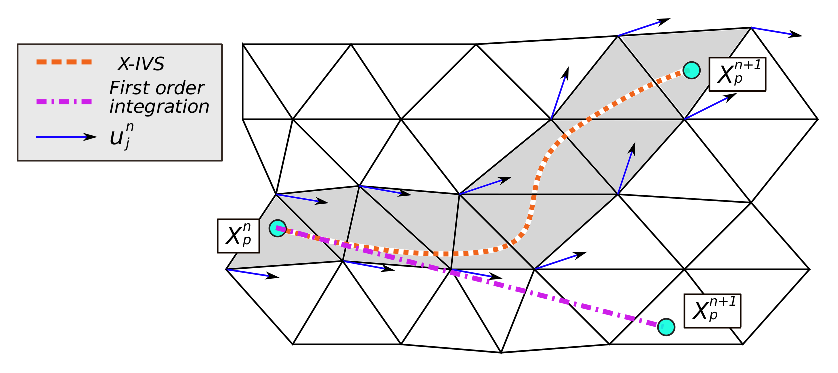
\includegraphics[scale=.6]{./imgs/xivs.eps}
\caption{Comparison of the trajectory of a particle moving from $x_q^n$ to $x_q^{n+1}$ for a given $\Delta t$ using the X-IVS method and a first order integration method. The vectors represent the fluid velocity at time $t^n$.}
\label{fig:xivs}
\end{figure}
%
In Fig.~\ref{fig:xivs} the trajectory of a particle is computed using the X-IVS method and it is compared to the trajectory of a first order integration scheme for a $CFL \gg 1$. 

Once the particles are moved to their new $t^{n+1}$ position the field $\phi$ that they transport (velocity, temperature, level set, etc.) needs to be mapped back to the mesh to perform the FEM analysis. Several approaches have been presented in \cite{gimenez:tesis}. In the current work the Global Least Squares Consistent (GLSC) methodology has been implemented and applied to our test cases. This approach solves a minimization problem where the approximation functions are the same linear shape functions used by the FEM discretization. This results in a global system where the unknowns are the nodal values. The minimization problem will be solved for $\phi$ such that it minimizes a global error function $E_g$ which computes the quadratic difference between the particle states $\phi_q$ at positions $\vect{x}_q$ surrounding a node at position $\vect{x}_j$ and the nodal value $\phi_j$:
%
\begin{equation}\label{eq:minim}
  E_g(\phi_1,\phi_2,...,\phi_j)=\frac{1}{2}\sum_{q=1}^{nq} \biggl(\phi_q-\sum_{j=1}^J\phi_jN_j(\vect{x}_q)\biggr)^2.
\end{equation}
%
To minimize $E_g$ Eq.~(\ref{eq:minim}) is derived with respect to $\phi_j$ and equaled to zero leading to the system of $J$ unknowns:
%
\begin{equation}\label{eq:mapptom}
  \vect{M}\vect{\phi}=\vect{f}
\end{equation}
%
where $J$ is the total number of nodes in the mesh, $\vect{M}_{ij}=\sum_qN_i(\vect{x}_q)N_j(\vect{x}_q)$ is a consistent mass matrix, $\vect{\phi}$ are the unknown nodal values and $\vect{f}_i=\sum_qN_i(\vect{x}_q)\phi_q$.

A step-by-step summary of the final algorithm for solving Navier-Stokes using fractional step and PFEM-2 is explained in Algorithm~\ref{algo:pfem2}.
%
\begin{algorithm}[H]
%\floatname{algorithm}{Fractional Step with PFEM-2}
\floatname{algorithm}{Algorithm}
%\renewcommand{\thealgorithm}{}
\caption{Summary of the steps needed for solving Navier-Stokes using fractional steps and PFEM-2.}
\label{algo:pfem2}
\begin{algorithmic}[1]
\STATE Compute the convection moving particles along streamlines (X-IVS)(Eq.~(\ref{xivs})).
\STATE Map particle velocities to mesh (Eq.~(\ref{eq:mapptom})).
\STATE Solve the system of Eqs.~(\ref{eq:masamat})-(\ref{eq:matunm2}) with $\beta=0$.
\STATE Correct velocity on particles (Eq.~(\ref{eq:partcor})).
\STATE Reseed particles if necessary.
\STATE Remove particles if allowed.
\end{algorithmic}
\end{algorithm} 
%
Another aspect of PFEM-2 which is more widely discussed in \cite{gimenez-difusion} is that of the particle inventory. Essentially it is the question of when, where and how to add or remove particles. In the present implementation particles are seeded into all the elements at initialization. There is a constant amount of particles per element at the beginning of a run. The number of initial particles can change for different problems. In this work all elements are seeded with twelve initial particles in 3D and nine in 2D. Since the objective of this paper is to evaluate the accuracy of PFEM-2 and compare it to that of FEM and experimental results then no strategy has been used to remove particles for the results presented later. The idea is to use PFEM-2 to its full accuracy capacity and removing particles is associated to a lose of accuracy by introducing numerical diffusion. Particles are added to the simulation to maintain a minimum amount of particles per element. This is a difference compared to \cite{gimenez-difusion} where the metric used to add particles is associated to the node. This will obviously decrease the computational performance of the simulation since the amount of particles will increase. The implementation relies on a robust parallel implementation to account for the increased demand of memory and CPU due to the increased number of particles. More on this subject will be explained in the next section. As an example to illustrate this issue a simple problem considering the flow past a 2D cylinder is used (see Fig.~\ref{fig:cyl_def}). It is better to use a 2D model for illustrative purposes. In Fig.~\ref{fig:cyl_evol} the initial configuration ``A'' is compared to an advanced configuration ``B''. Initially all elements have the same amount of particles and the distribution is homogeneous. As the flow evolves particles agglomerate increasing the overall amount of particles in the domain. Finally Fig.~\ref{fig:cyl_npart} shows a curve with the number of particles as a function of time. Note how the number of particles increase rapidly at the beginning of the simulation and then reaches a pseudo-steady state amount. The objective of future implementations will be to attempt to maintain a constant number of particles while preserving the accuracy of the method. There is more about the particle inventory implications for parallel implementations in the next section.
%
\begin{figure}[htp] 
\centering 
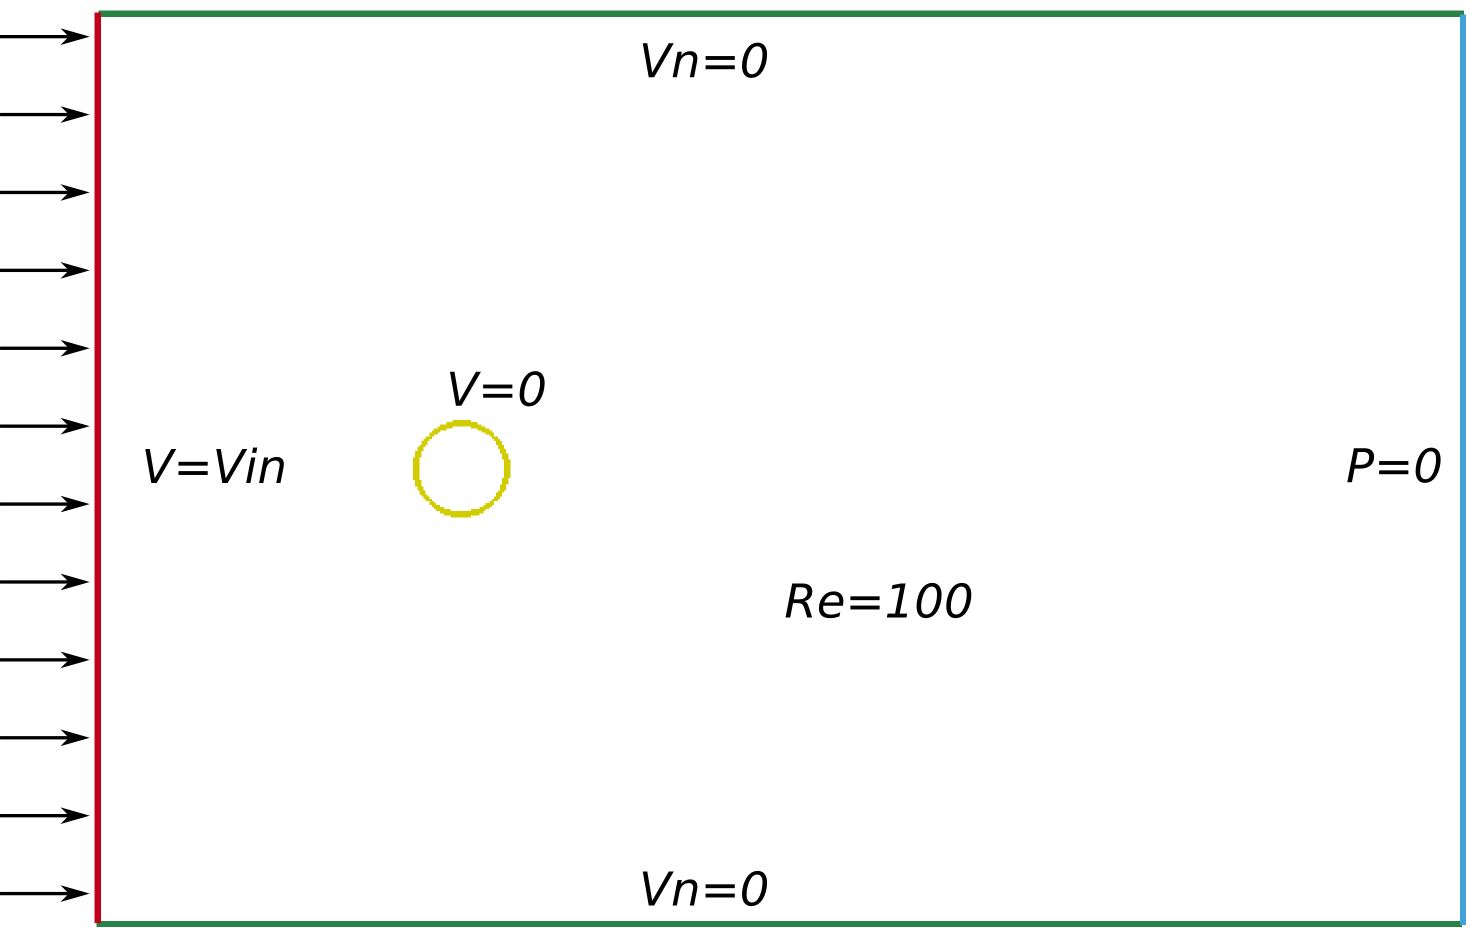
\includegraphics[scale=.5]{./imgs/cyl_def.png}
\caption{Problem definition for the 2D cylinder problem and boundary conditions.}
\label{fig:cyl_def}
\end{figure}
%
\begin{figure}[htp]
\centering 
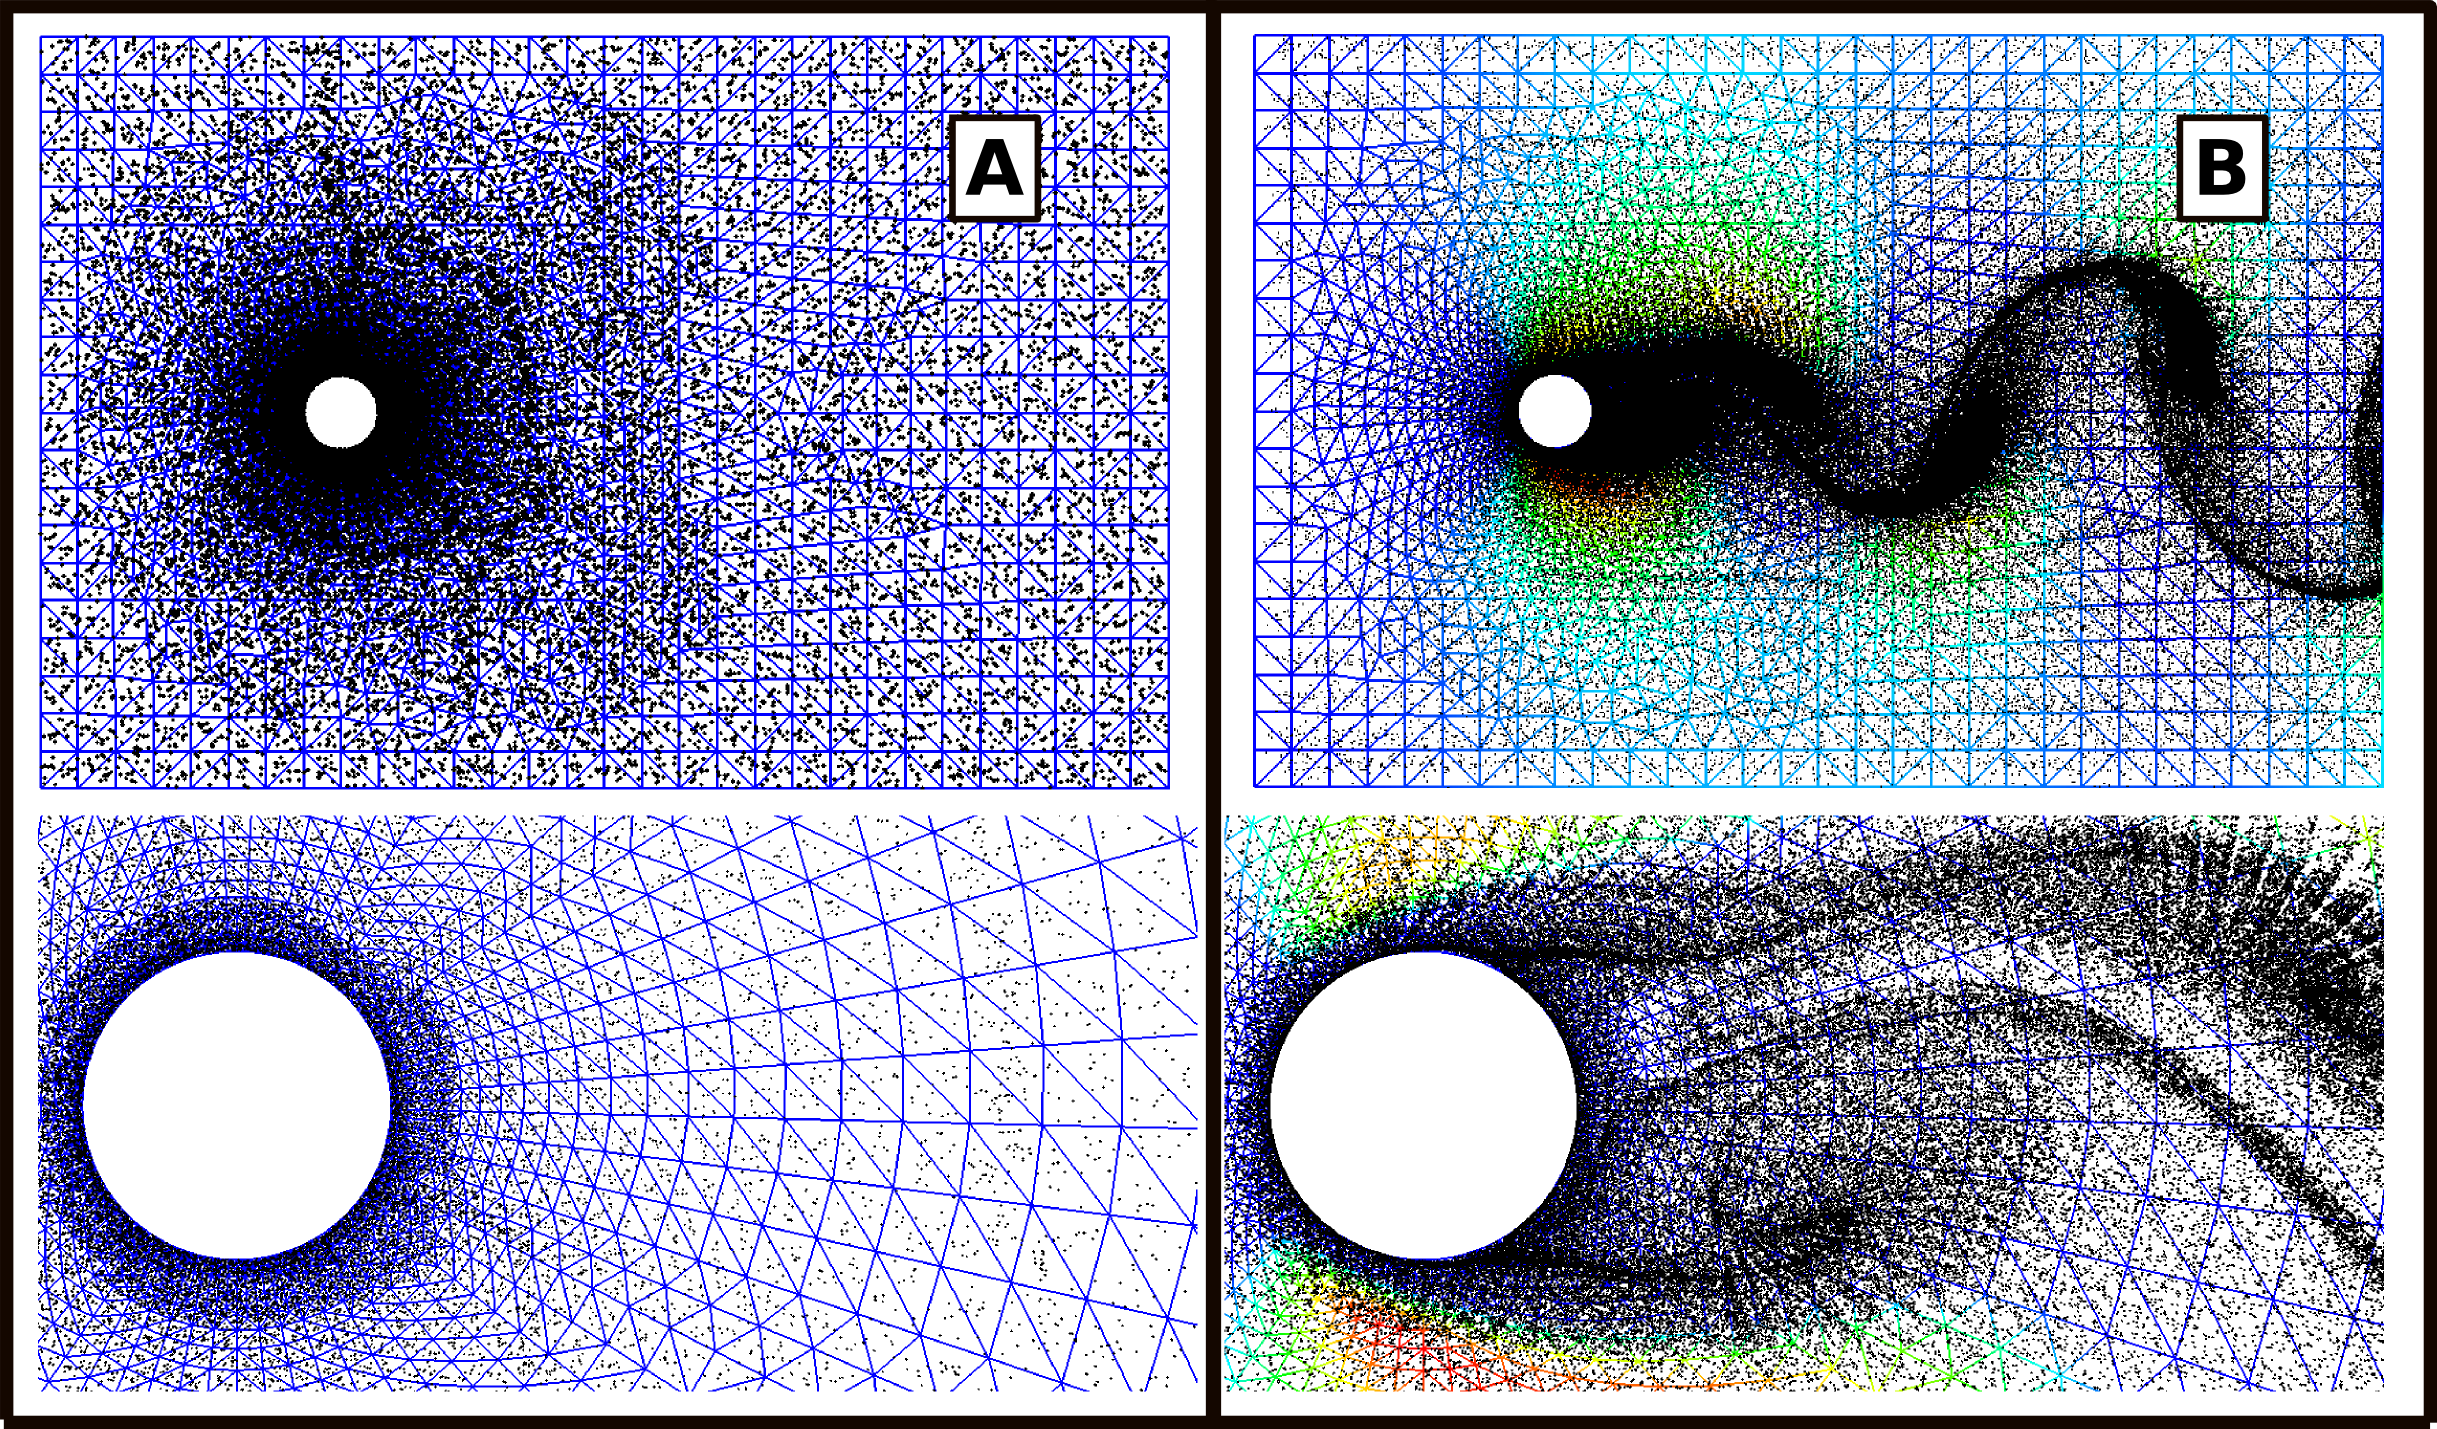
\includegraphics[scale=.4]{./imgs/cyl_parts.png}
\caption{Evolution of particle position and number of particles for the 2D cylinder problem. A) Initial configuration and B) advanced particle configuration.}
\label{fig:cyl_evol}
\end{figure}
%
\begin{figure}[htp] 
\centering 
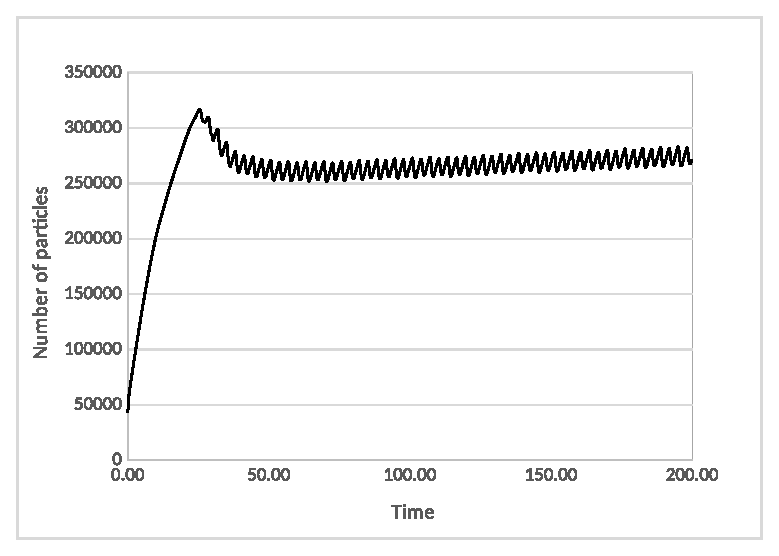
\includegraphics[scale=.6]{./imgs/npart_cyl_excel.eps}
\caption{Number of particles as a function of a non-dimensional time for the cylinder problem. Observe how to particle number increase rapidly and then they reach a pseudo-steady state amount.}
\label{fig:cyl_npart}
\end{figure}

 \subsection{Parallel Implementation}
  The parallel implementation for PFEM-2 follows the guidelines presnted in \cite{gimenez:parallel} for the case of distributed memory architectures. The challenges are well described in their paper but basically involves the extra amount of memory needed for the particle data structure. Due to the explicit scheme the parallel implementation needs to take care of local operations to each particle separately from the rest allowing for trivial parallelization. The dificulty arise at the interface between processors where particles may travel several elements and possible processors before finding their final host element. This task requieres an outer loop to communicate particles that will terminate when no more particles cross the interface between partitions. In figure \ref{fig:parallel} there is an illustration of how particles may move across processors. The thick black line depicts the partition. In the first case a particle lands in the same processor which involves no communication. In the second case a particle moves across a single interface and communication takes place. In the third place a particle may move accross two or more processors in which case the outer loop will perform as many communications as necessary untill no more particles cross a processor interface.

\begin{figure}[htp] 
\centering 
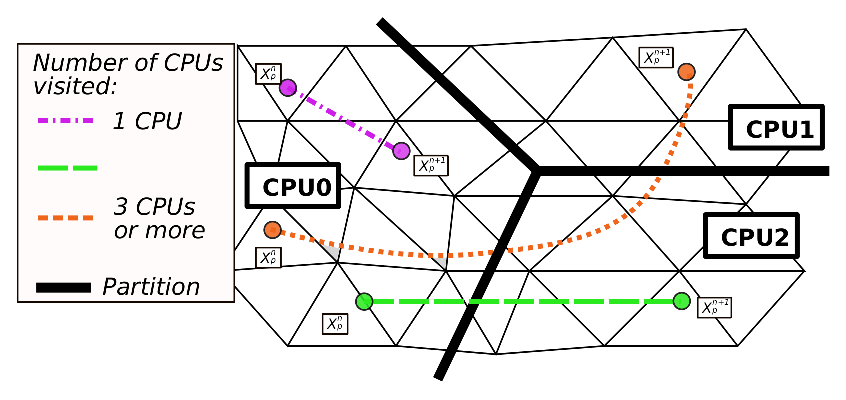
\includegraphics[scale=.4]{./imgs/parallel.eps}
\caption{Different ways that particles may move across processor interfaces.}
\label{fig:parallel}
\end{figure}


The current approach is built ``on top'' of a pre-existing parallel FEM implementation thus inheriting much of the data structures and methodologies. The partitions are creating using the software METIS \cite{metis1,metis}...

In the present implementation load balancing has not being address. Extrictely speaking if particles are not removed at some point accumulation of particles in one partition will be an issue. This is something that will be address later. Most luckily the PFEM-2 impliementation will change to allow removal of particles in such a way that an almost constant amount of particles is preserved at each element. The techniques for particle inventory presented in \cite{gimenez-difusion} will be implemented.



[IMAGE WITH PARTICLES MOVING THROUGH PARTITIONS]



[IMAGE SCALABILITY]


 


\section{Numerical results}
% intro 
The simulations of blood flows in a nozzle, pump, and IVC with FEM and PFEM-2 are conducted and compared with experimental results \cite{fda_res,fda_nozzle ,fda_pump,gallagher_exp}. The fluid is assumed to be blood analog Newtonian fluid. For the nozzle and pump flows, the fluid density and viscosity are set to be $\rho= 1035$ kg/m\textsuperscript{3} and $\mu =3.5\times10^{-3}$ N-s/m\textsuperscript{2}, where as for the IVC flows, the density and viscosity are $\rho=1817$ kg/m\textsuperscript{3}, $\mu=5.83\times10^{-3}$ N-s/m\textsuperscript{2} for resting condition and $\mu=5.49\times10^{-3}$ N-s/m\textsuperscript{2} for exercising condition. 

\subsection{Blood Nozzle}

%  nozzle intro
The simplified nozzle proposed by FDA consists of four parts containing characteristics of some blood-conveying medical devices. There are inlet and outlet tubes with diameter $0.012$ m, as well as a cone-shaped converging tube connecting the inlet tube with the nozzle throat with diameter $0.004$ m as shown in Fig.~\ref{fig:nozzlegeo1}. The flow experiences a gradual contraction of area from the inlet tube to the throat, then a sudden expansion of area right after the throat to the outlet tube (see Fig.~\ref{fig:nozzlegeo2}). The z coordinate along the axial direction has origin at the exit of the nozzle throat. The flow at Reynolds number $3500$ with flowrate $3.64\times10^{-5}$ m\textsuperscript{3}/s corresponding to turbulent flow regime is analyzed, where the Reynolds number is defined with the flow rate and the diameter at the throat. 

*** ADD COMPUTATIONAL DOMAIN TO SHOW THAT IT IS A 3D MODEL ***

%% PEGGY: should these geometry figures be included?
\begin{figure}[htbp]
    \centering
    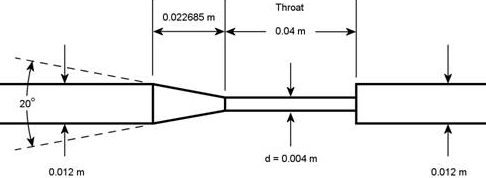
\includegraphics[width=3.3in]{imgs/nozzle_pump/nozzle_geo_2.png}
    \caption{The dimension of the idealized nozzle model proposed by FDA.}
    \label{fig:nozzlegeo1}
\end{figure}
\begin{figure}[htbp]
    \centering
    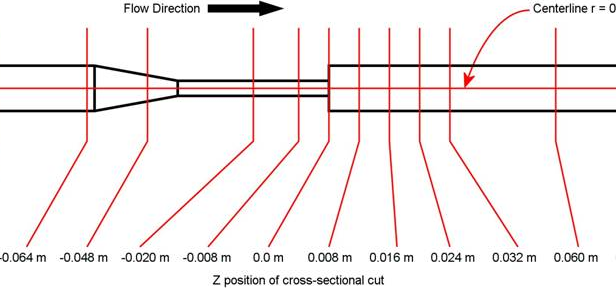
\includegraphics[width=3.3in]{imgs/nozzle_pump/nozzle_CS_2.png}
    \caption{The flow direction and the definition of the axial coordinate z.}
    \label{fig:nozzlegeo2}
\end{figure}


%  nozzle simulation setup
For the set up of the numerical simulation a 3D domain is defined from $z=-0.18$ m to $z=0.18$ m. The prescribed uniformly distributed velocity profile is imposed at the inlet while the pressure is constant at outlet. The Large Eddy Simulation (LES) Smagorinsky model is chosen to deal with the turbulence regime in the nozzle, and the Smagorinsky coefficient is set to be $0.1$ (empirically derived for flows in pipes). The turbulence intensity at the inlet is set to be $5$\% (see Smirnov's turbulence synthesis method~\cite{Smirnov2001}). There are two different kinds of meshes considered in this study: mesh A with a more uniform mesh size in the outlet tube, and mesh B has mesh refinement at certain area (see Fig.~\ref{fig:nozzlemesh}). The mesh A has minimum mesh size $0.2$ mm and a total of $8.61$M elements. The mesh B has mostly coarser elements in the outlet tube than mesh A, but with mesh refinement near the exit of the throat. The minimum mesh size of mesh B is $0.1$ mm with total of $1.13$M elements. By using two distinct meshes the sensitivity of the FEM and PFEM-2 methods to the mesh resolution may be observed. Simulations with different CFL number will also be done to examine the influence of the time step size with these two methods.

\begin{figure}[htbp]
    \centering
    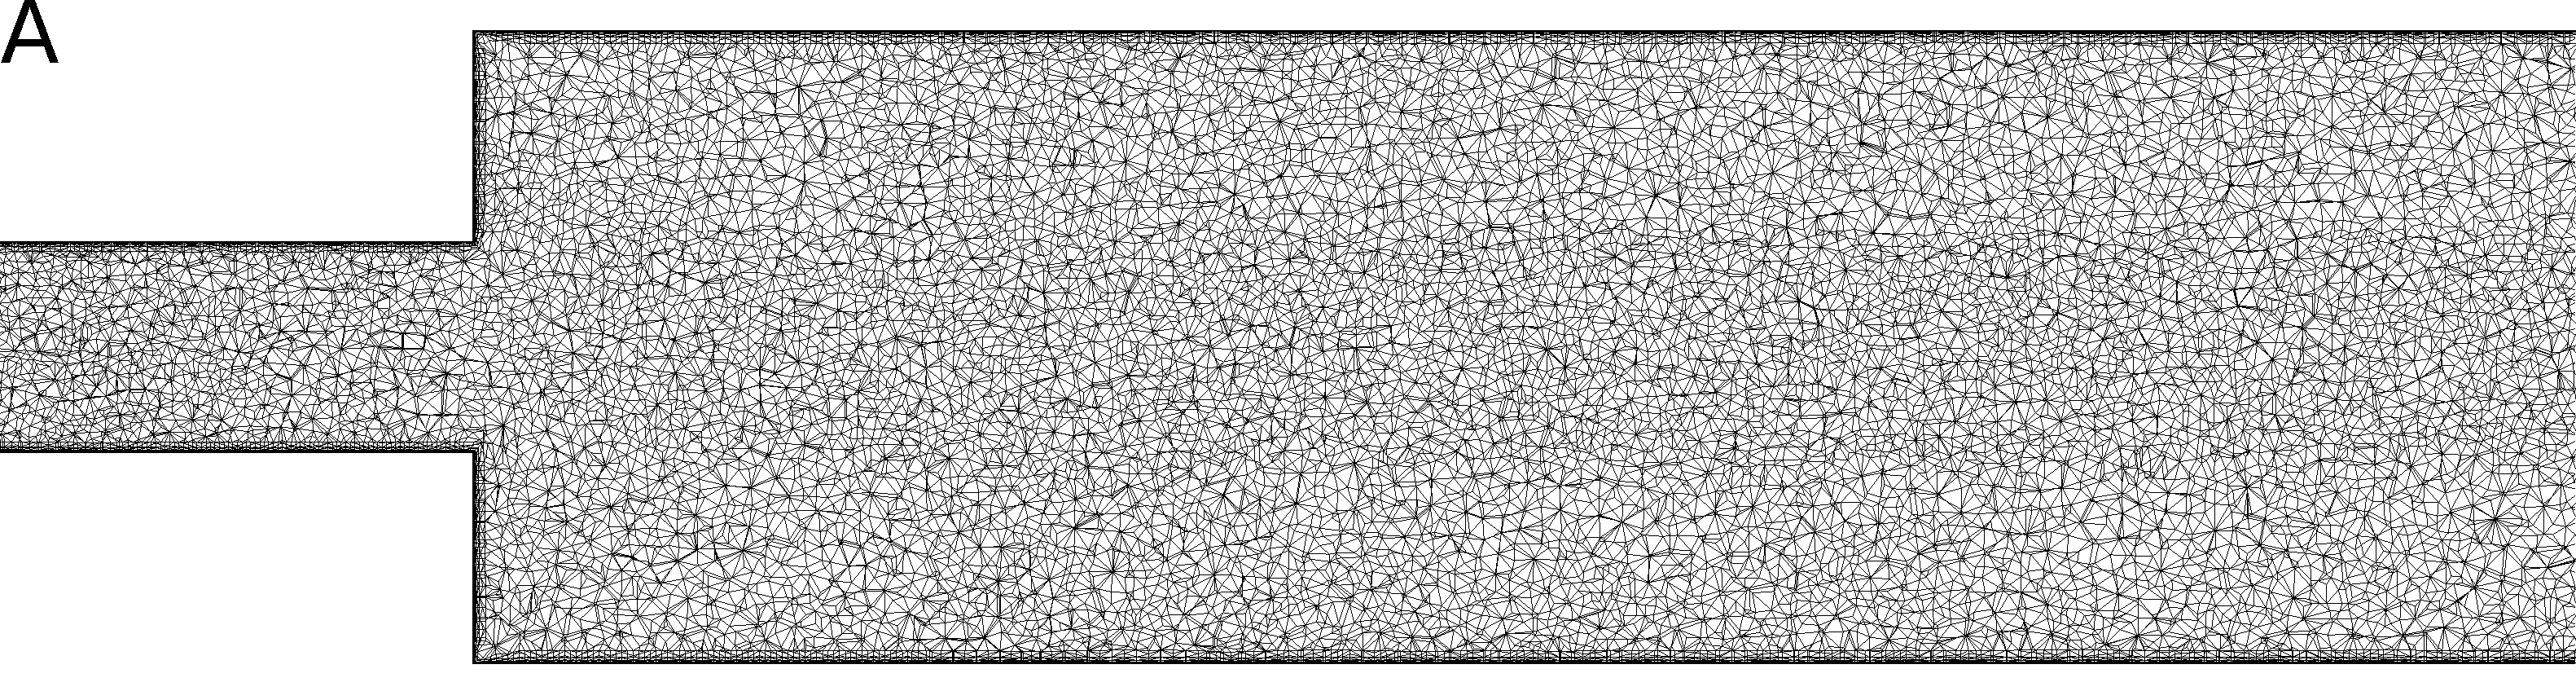
\includegraphics[width=3.2in]{imgs/nozzle_pump/nozzle_fmesh_2.pdf}
    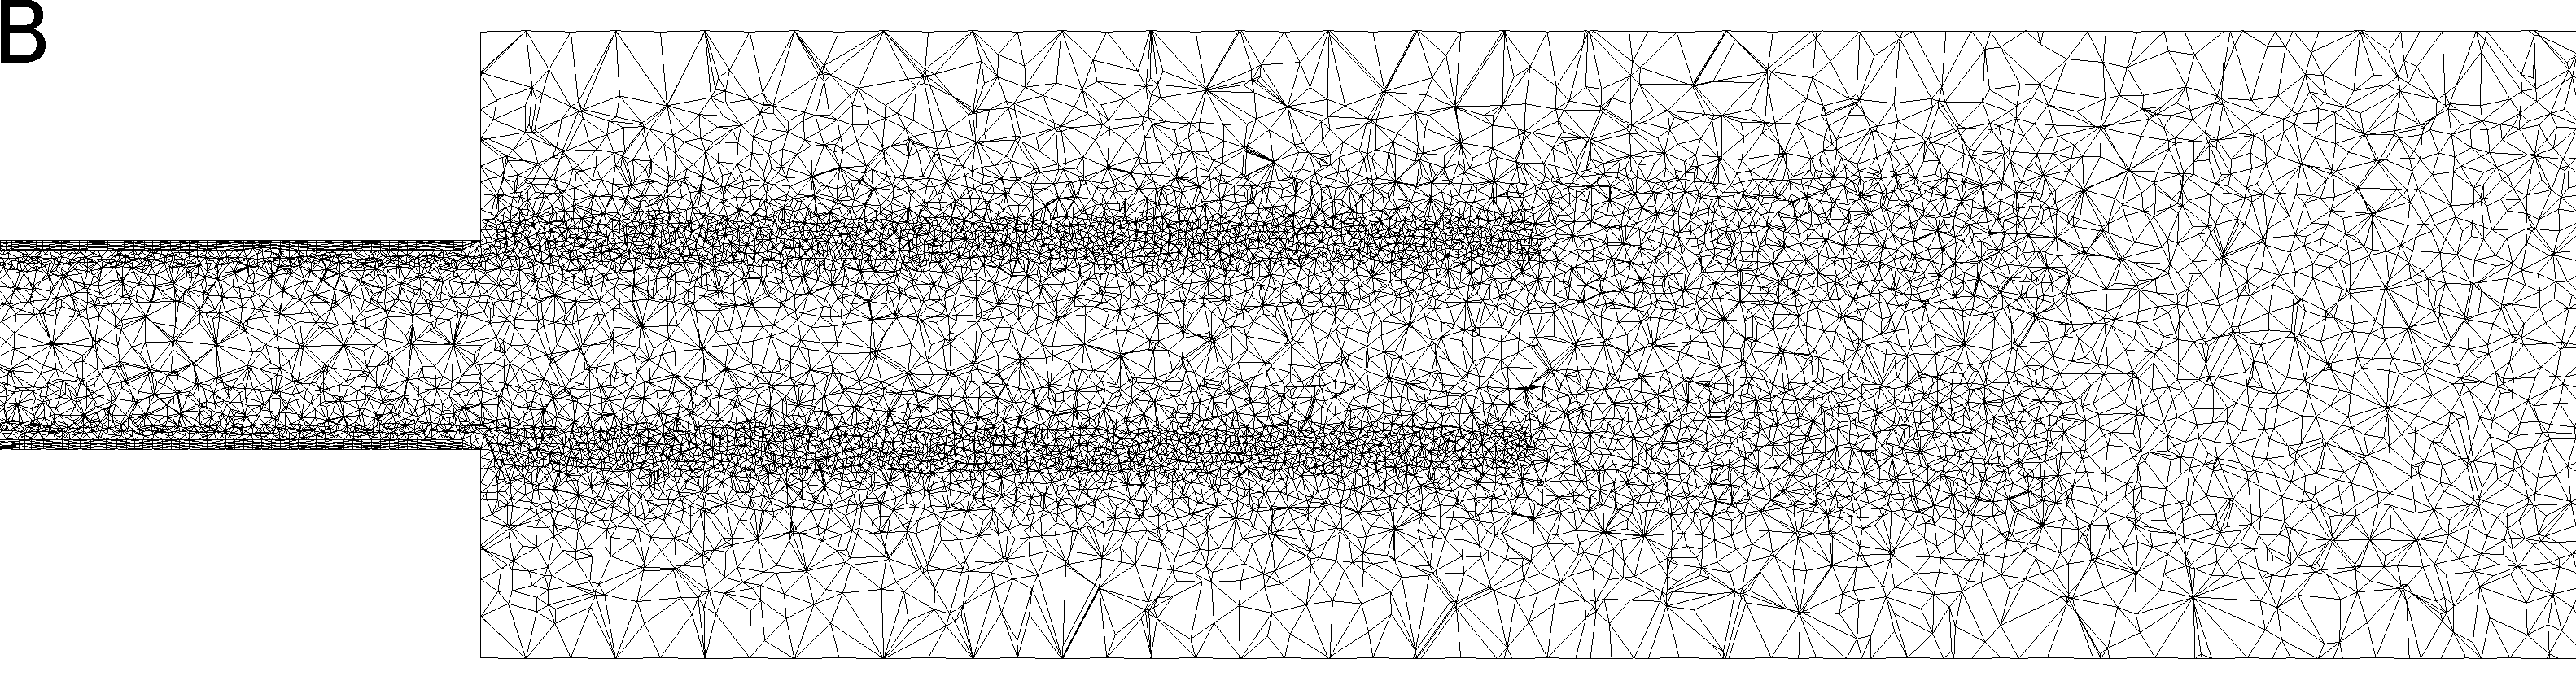
\includegraphics[width=3.2in]{imgs/nozzle_pump/nozzle_pmesh_2.pdf}
    \caption{The two meshes A (top) and B (bottom) used in the blood nozzle simulations.}
    \label{fig:nozzlemesh}
\end{figure}

% nozzle result and analysis

The obtained distributions of the time average velocity magnitude in the nozzle after reaching steady state are shown in Figs. \ref{fig:nozzlevelfm} and \ref{fig:nozzlevelpm}. It can be observed that the sudden expansion at the exit of the throat leads to the formation of a jet. In turbulent regime, the center velocity of the jet has a sudden decrease called jet breakdown. Most of the obtained results show the breakdown of the jet, but with different breakdown locations. This can be shown clearly in Fig.~\ref{fig:nozzlemidvel} which illustrates the time average velocity along the center line of the nozzle, where the origin of the axial coordinate is at the exit of the throat (Fig.~\ref{fig:nozzlegeo2}). It can be observed that results by PFEM-2 all have good agreement with experiments in \cite{hariharan_nozzle} with both meshes. Also, the results using PFEM-2 are not affected much by the time step size. Note that the result of PFEM-2 using a $CFL=10$ shows an apparent closer agreement between the numerical result and the experiment. This does not imply that a larger time step better predicts the numerical solution but rather that this solution is within the statistical dispersion of the method. A further statistical analysis (which is outside of the scope of this paper) could help quantify the spread of the solution when the time steps increase. On the other hand, for the results using FEM, the estimated breakdown locations of the jet are affected largely when the CFL number is larger than 1. Additionally the breakdown locations are also affected by the mesh configuration. For the FEM mesh B clearly provides a better solution than mesh A while the solution by PFEM-2 does not show a substantial difference. The reason why mesh B is superior in the FEM is that in the regions with higher velocity gradients the mesh has a higher resolution decreasing the numerical viscosity added in the velocity stabilization term. 

\begin{figure}[htbp]
    \centering
    FEM\\
    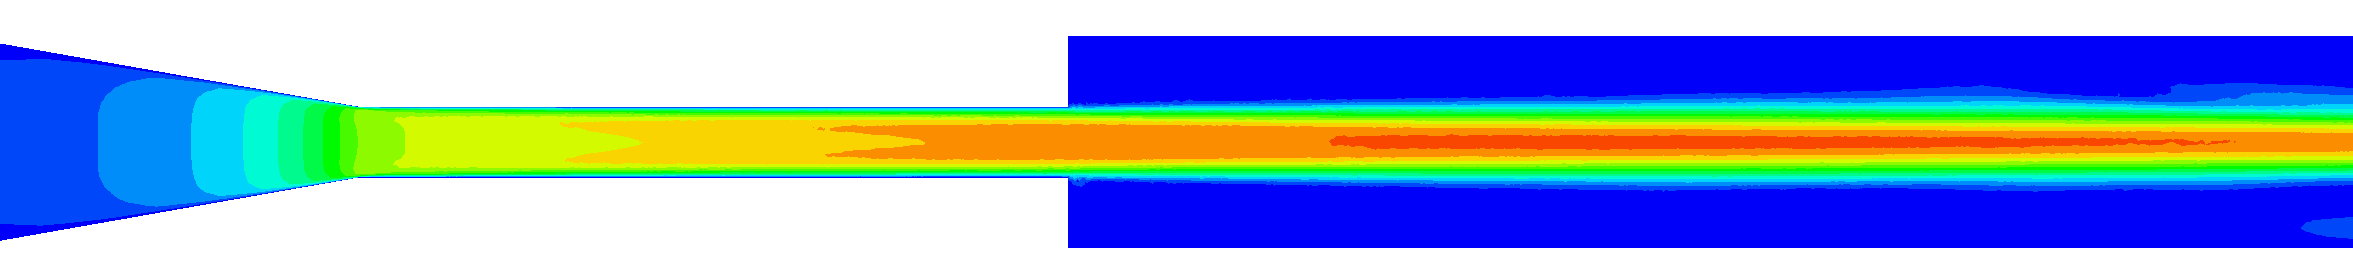
\includegraphics[width=3.2in]{imgs/nozzle_pump/nozzle_fem_fm_cfl1.png}
    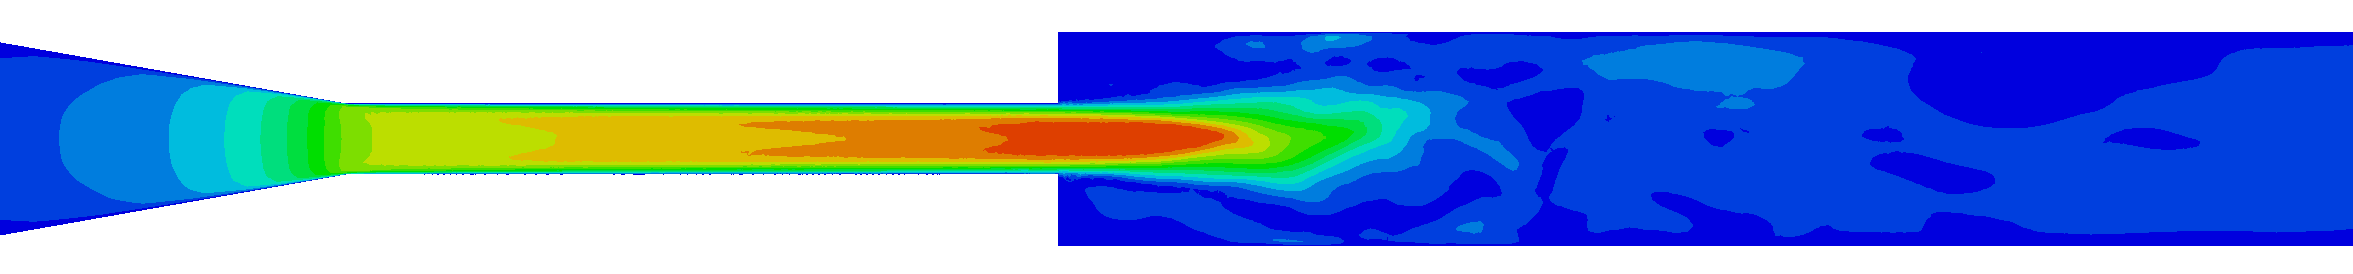
\includegraphics[width=3.2in]{imgs/nozzle_pump/nozzle_fem_fm_cfl5.png}\\
    PFEM-2\\
    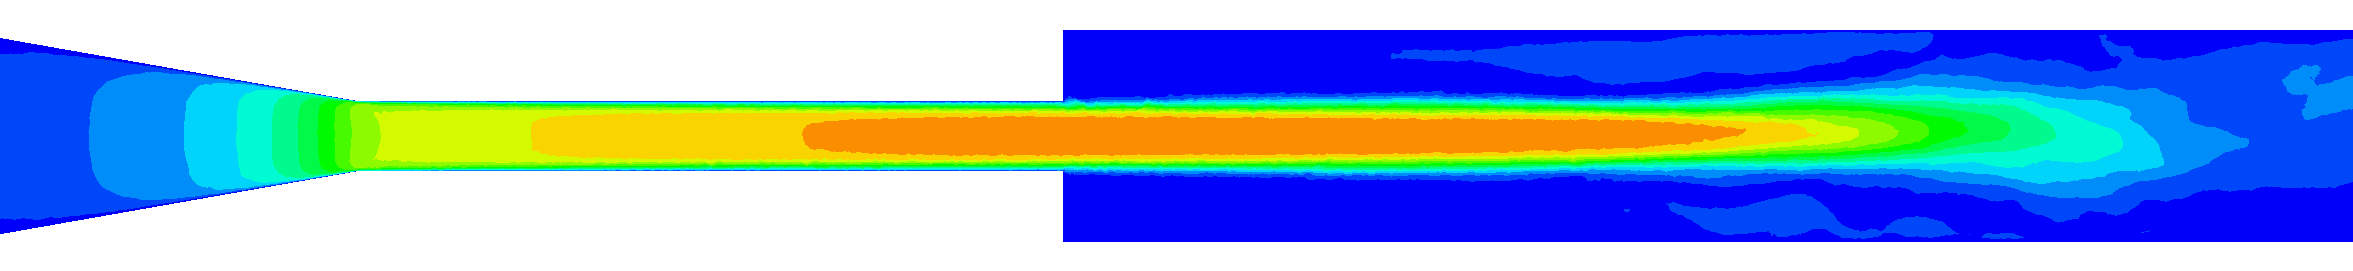
\includegraphics[width=3.2in]{imgs/nozzle_pump/nozzle_pfem_fm_cfl1.png}
    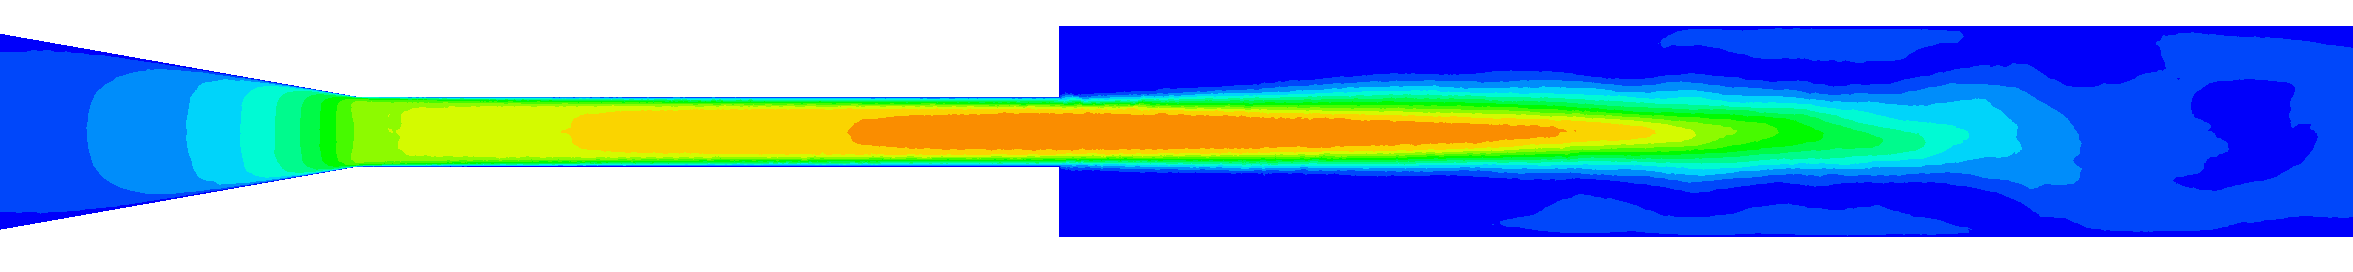
\includegraphics[width=3.2in]{imgs/nozzle_pump/nozzle_pfem_fm_cfl5.png}
    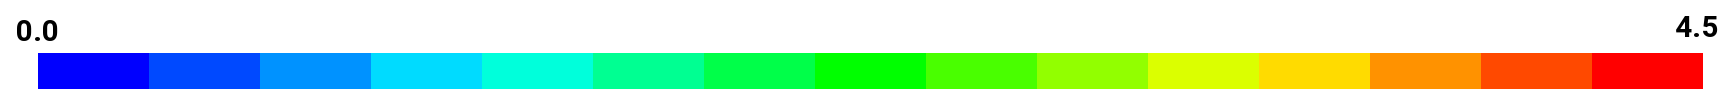
\includegraphics[width=3.2in]{imgs/nozzle_pump/nozzle_legend.png}
    \caption{The obtained time average velocity magnitude distribution in the nozzle at steady state with mesh A using FEM and PFEM-2 with CFL=1 (1st and 3rd plots) and CFL=10 (2nd and 4th plots). }
    \label{fig:nozzlevelfm}
\end{figure}

\begin{figure}[htbp]
    \centering
    FEM\\
    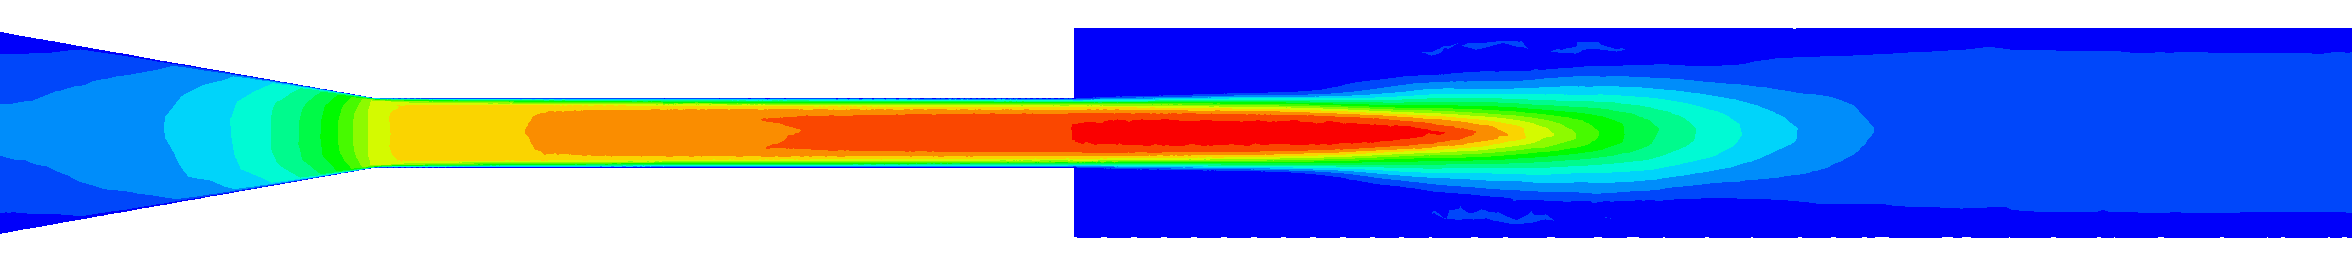
\includegraphics[width=3.2in]{imgs/nozzle_pump/nozzle_fem_pm_cfl1.png}
    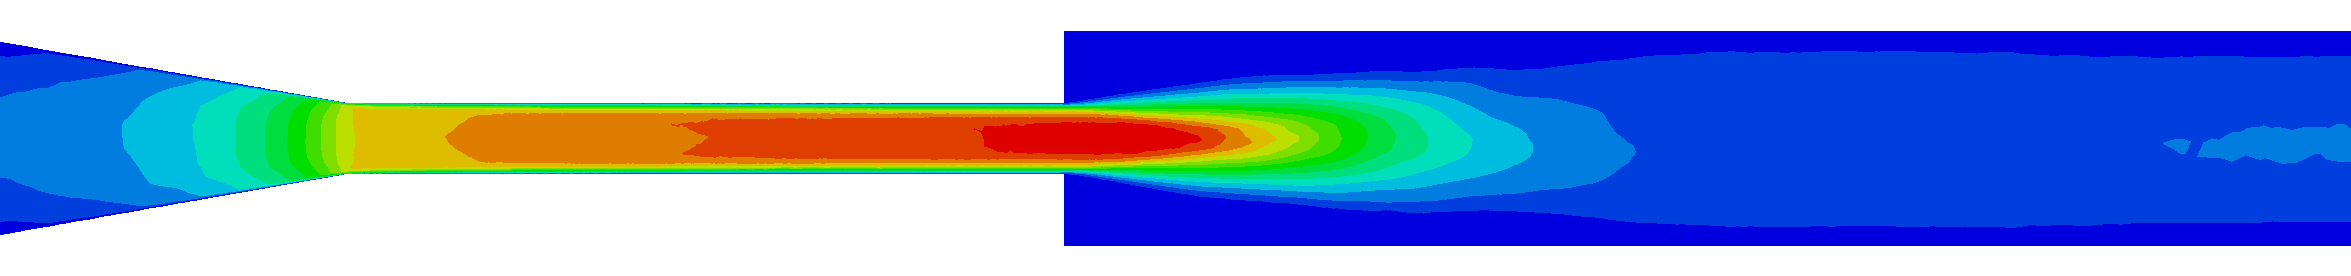
\includegraphics[width=3.2in]{imgs/nozzle_pump/nozzle_fem_pm_cfl10.png}
    PFEM-2\\
    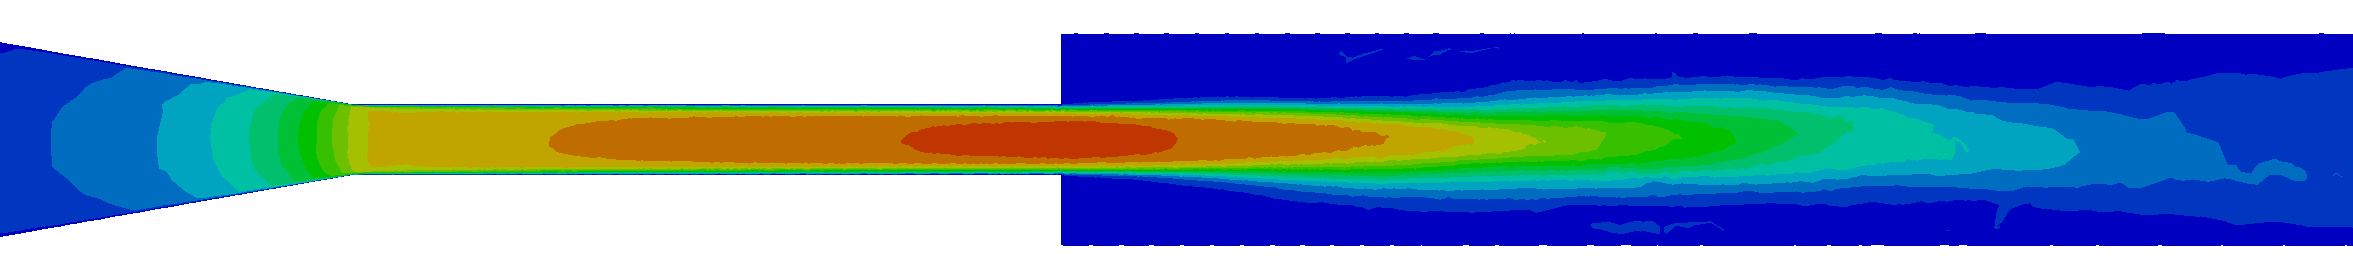
\includegraphics[width=3.2in]{imgs/nozzle_pump/nozzle_pfem_pm_cfl1.png}
    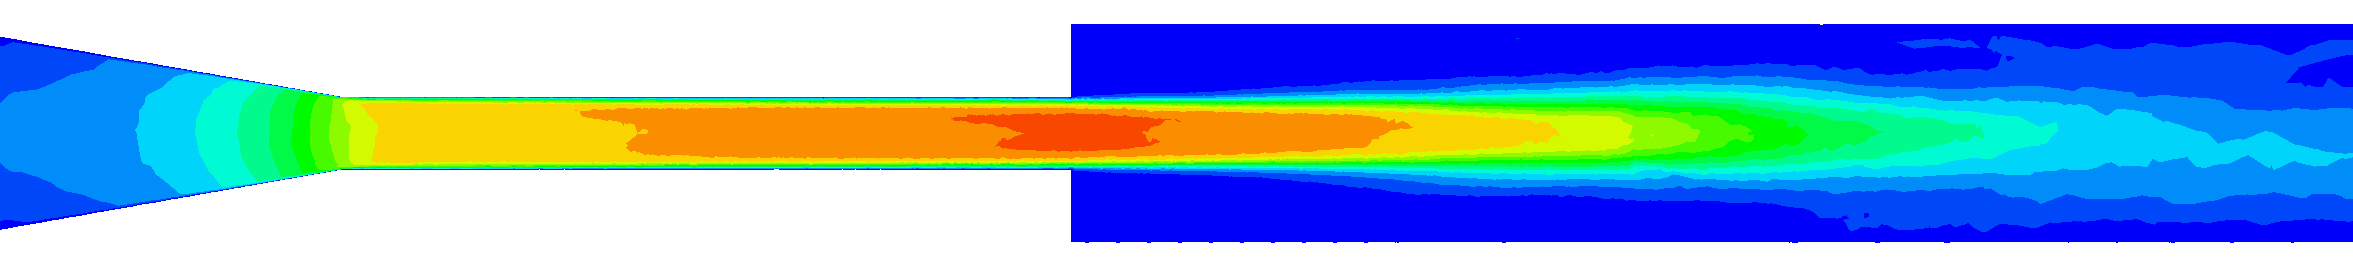
\includegraphics[width=3.2in]{imgs/nozzle_pump/nozzle_pfem_pm_cfl10.png}
    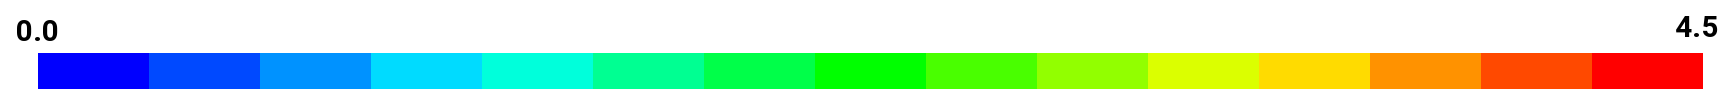
\includegraphics[width=3.2in]{imgs/nozzle_pump/nozzle_legend.png}
    \caption{The obtained time average velocity magnitude distribution in the nozzle at steady state with mesh B using FEM and PFEM-2 with CFL=1 (1st and 3rd plots) and CFL=10 (2nd and 4th plots).}
    \label{fig:nozzlevelpm}
\end{figure}


\begin{figure}[htbp]
    \centering
    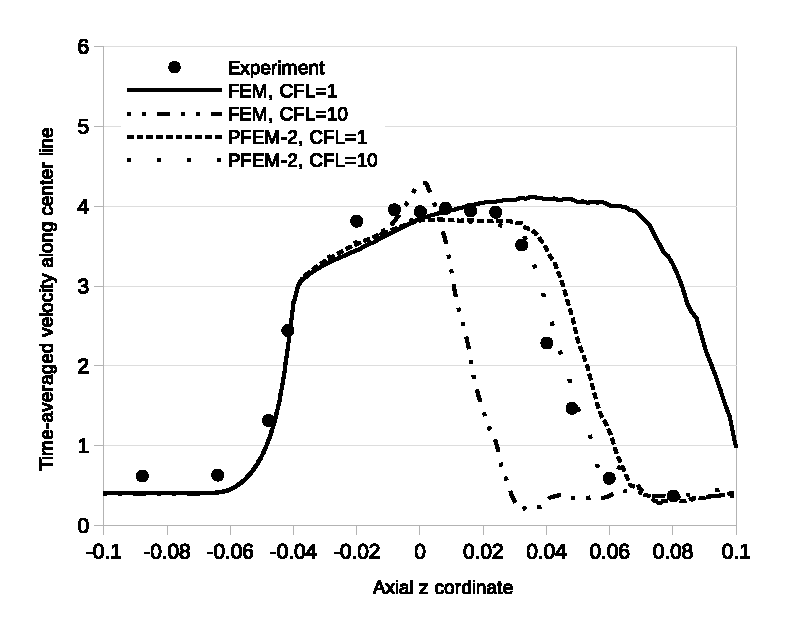
\includegraphics[width=3.2in]{imgs/nozzle_pump/nozzle_midvel_fm2.eps}
    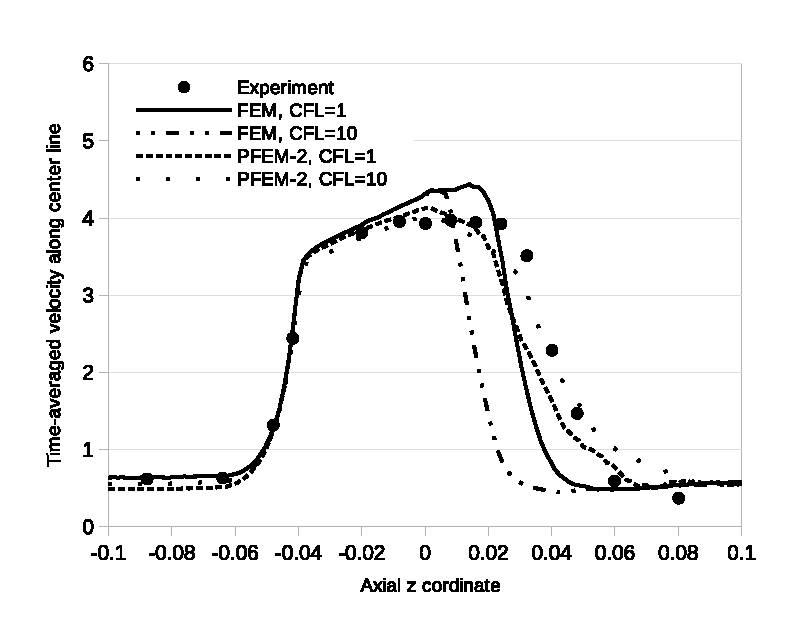
\includegraphics[width=3.2in]{imgs/nozzle_pump/nozzle_midvel_pm2.eps}
    \caption{The distribution of the axial velocity in the nozzle along the center line with mesh A (top) and mesh B (bottom).
%The distribution of the axial velocity in the nozzle along the center line. The top figure depicts the results with mesh A using FEM and CFL=1 (solid), FEM and CFL=5 (dash-dotted), PFEM-2 and CFL=1 (dashed) and PFEM2 and CFL=5 (dotted). The bottom figure depicts the results with mesh B using FEM and CFL=1 (solid), FEM and CFL=10 (dash-dotted), PFEM-2 and CFL=1 (dashed) and PFEM2 and CFL=10 (dotted).
}
    \label{fig:nozzlemidvel}
\end{figure}

\subsection{Blood Pump}

%  pump intro
The geometry of the FDA proposed simplified centrifugal pump is shown in the Fig.~\ref{fig:pumpgeo}. The flow enters the chamber through a curved tube with diameter $12$ mm. The diameter of the inner chamber of the housing is $60$ mm and the thickness is $9$ mm. The rotor inside the chamber has a diameter of $52$ mm and $4$ mm thick, along with four $3$ mm thick straight blades. The chamber is connected with a throat at its outlet, followed by a diffuser to the outlet tube with diameter $12$ mm. The pump flow with flowrate $Q=6$ L/min and rotational speed $3500$ RPM is analyzed. 

%% PEGGY: should these geometry figures be included?
\begin{figure}[htbp]
    \centering
    \begin{minipage}[c][2.5in][c]{0.9\linewidth}
        \centering
        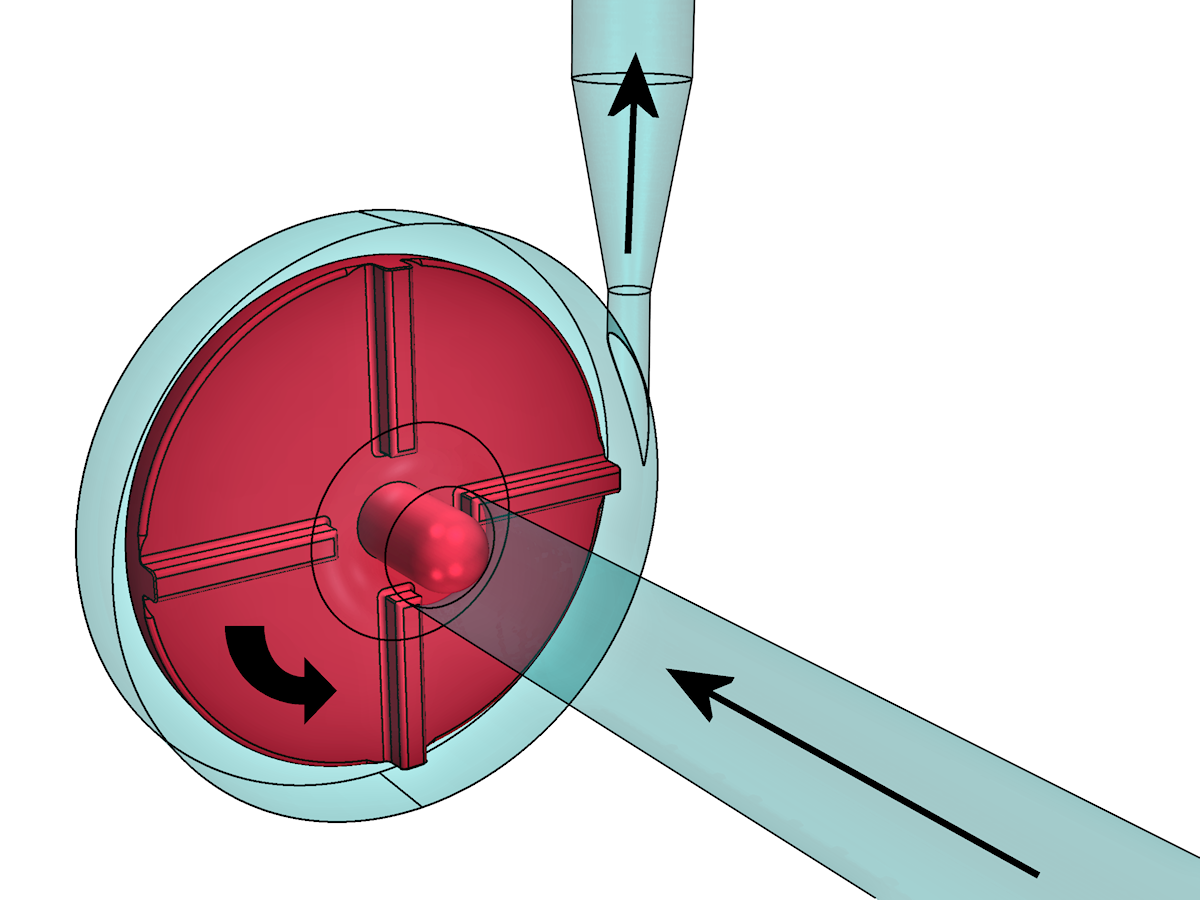
\includegraphics[width=3.2in]{imgs/nozzle_pump/housing_and_rotor.png}
    \end{minipage}
    \begin{minipage}[c][2.5in][c]{0.9\linewidth}
        \centering
        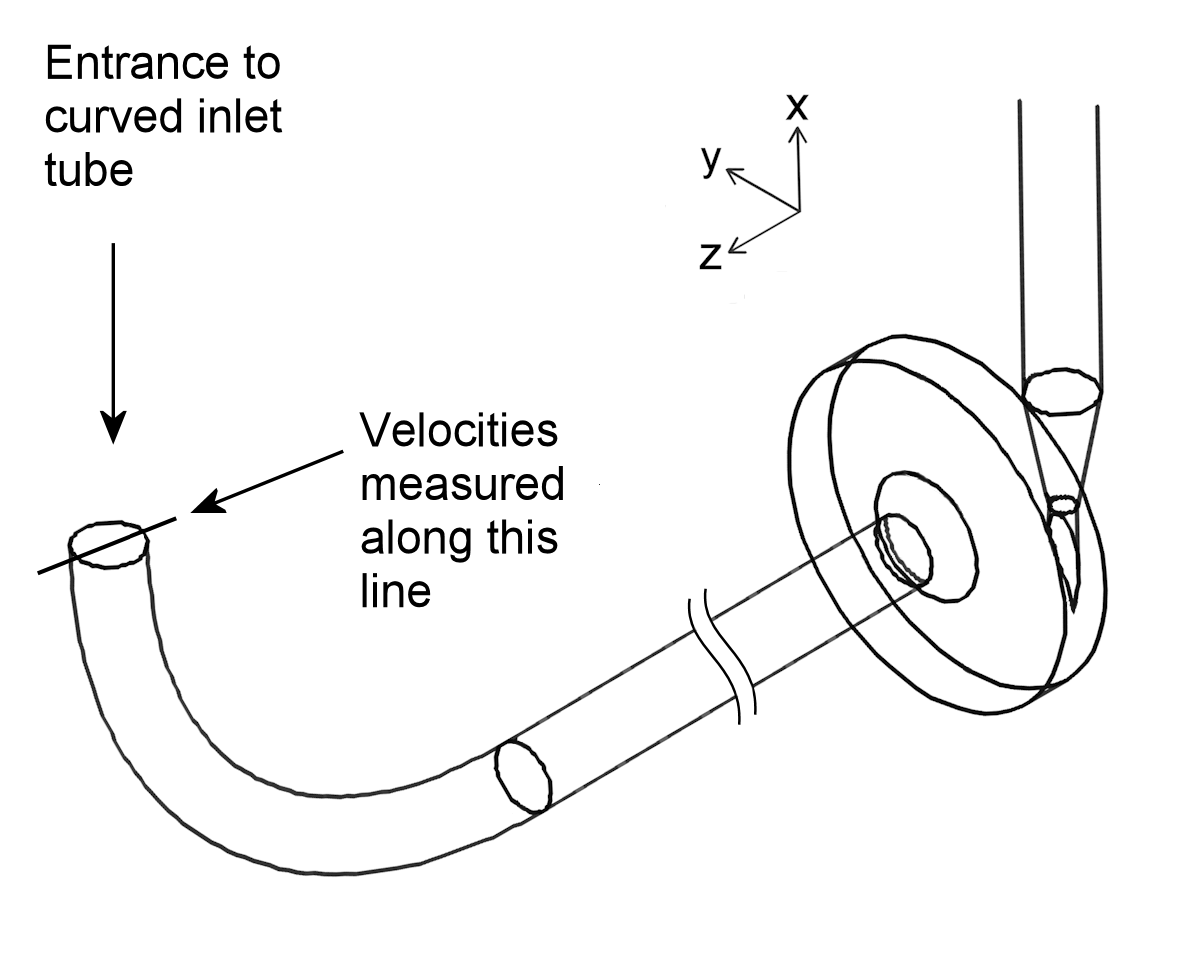
\includegraphics[width=3.2in]{imgs/nozzle_pump/inlet_velcocity_profile_location.png}
    \end{minipage}
    \caption{The pump geometry and the flow direction in the blood pump (top), and the inlet location where the velocity is measured in experiments and where the velocity profile is prescribed in the simulations (bottom).}
    \label{fig:pumpgeo}
\end{figure}

%  pump simulation setup
As to the simulation set up, the velocity distribution is prescribed at the inlet (Fig.~\ref{fig:pumpgeo}), where the velocity profiles are obtained from the experimental measurements using PIV \cite{cpi}. The pressure at the outlet is set to be constant. Since the goal is to predict the flow field after reaching steady state, instead of letting the rotor rotate during simulation, the non-inertial reference frame is applied on the fluid around the rotor. This is because the flow around the rotor at steady state can be analogue to flow experiencing constant angular velocity. Using non-inertial reference frame approximation avoids mesh distortion and frequent remeshing due to rotation. The LES Wall-Adapting Local Eddy-viscosity (WALE) \cite{wale} turbulence model is employed. 

The simulation domain is decomposed into around $1$ million tetrahedron elements. The mesh size is $0.5$ mm on the rotor blades and $0.3$ mm at the outlet of the chamber to the diffuser. The mesh is locally refined around the throat as shown in Fig.~\ref{fig:pumpmesh}. The simulation result is obtained after $8$ rotations when the pump flow already reaches steady state. The time step size is around $10^{-5}$ s in FEM and PFEM-2 simulations at steady state so that the CFL number is less or equal than $1$.  
\begin{figure}[htbp]
    \centering
    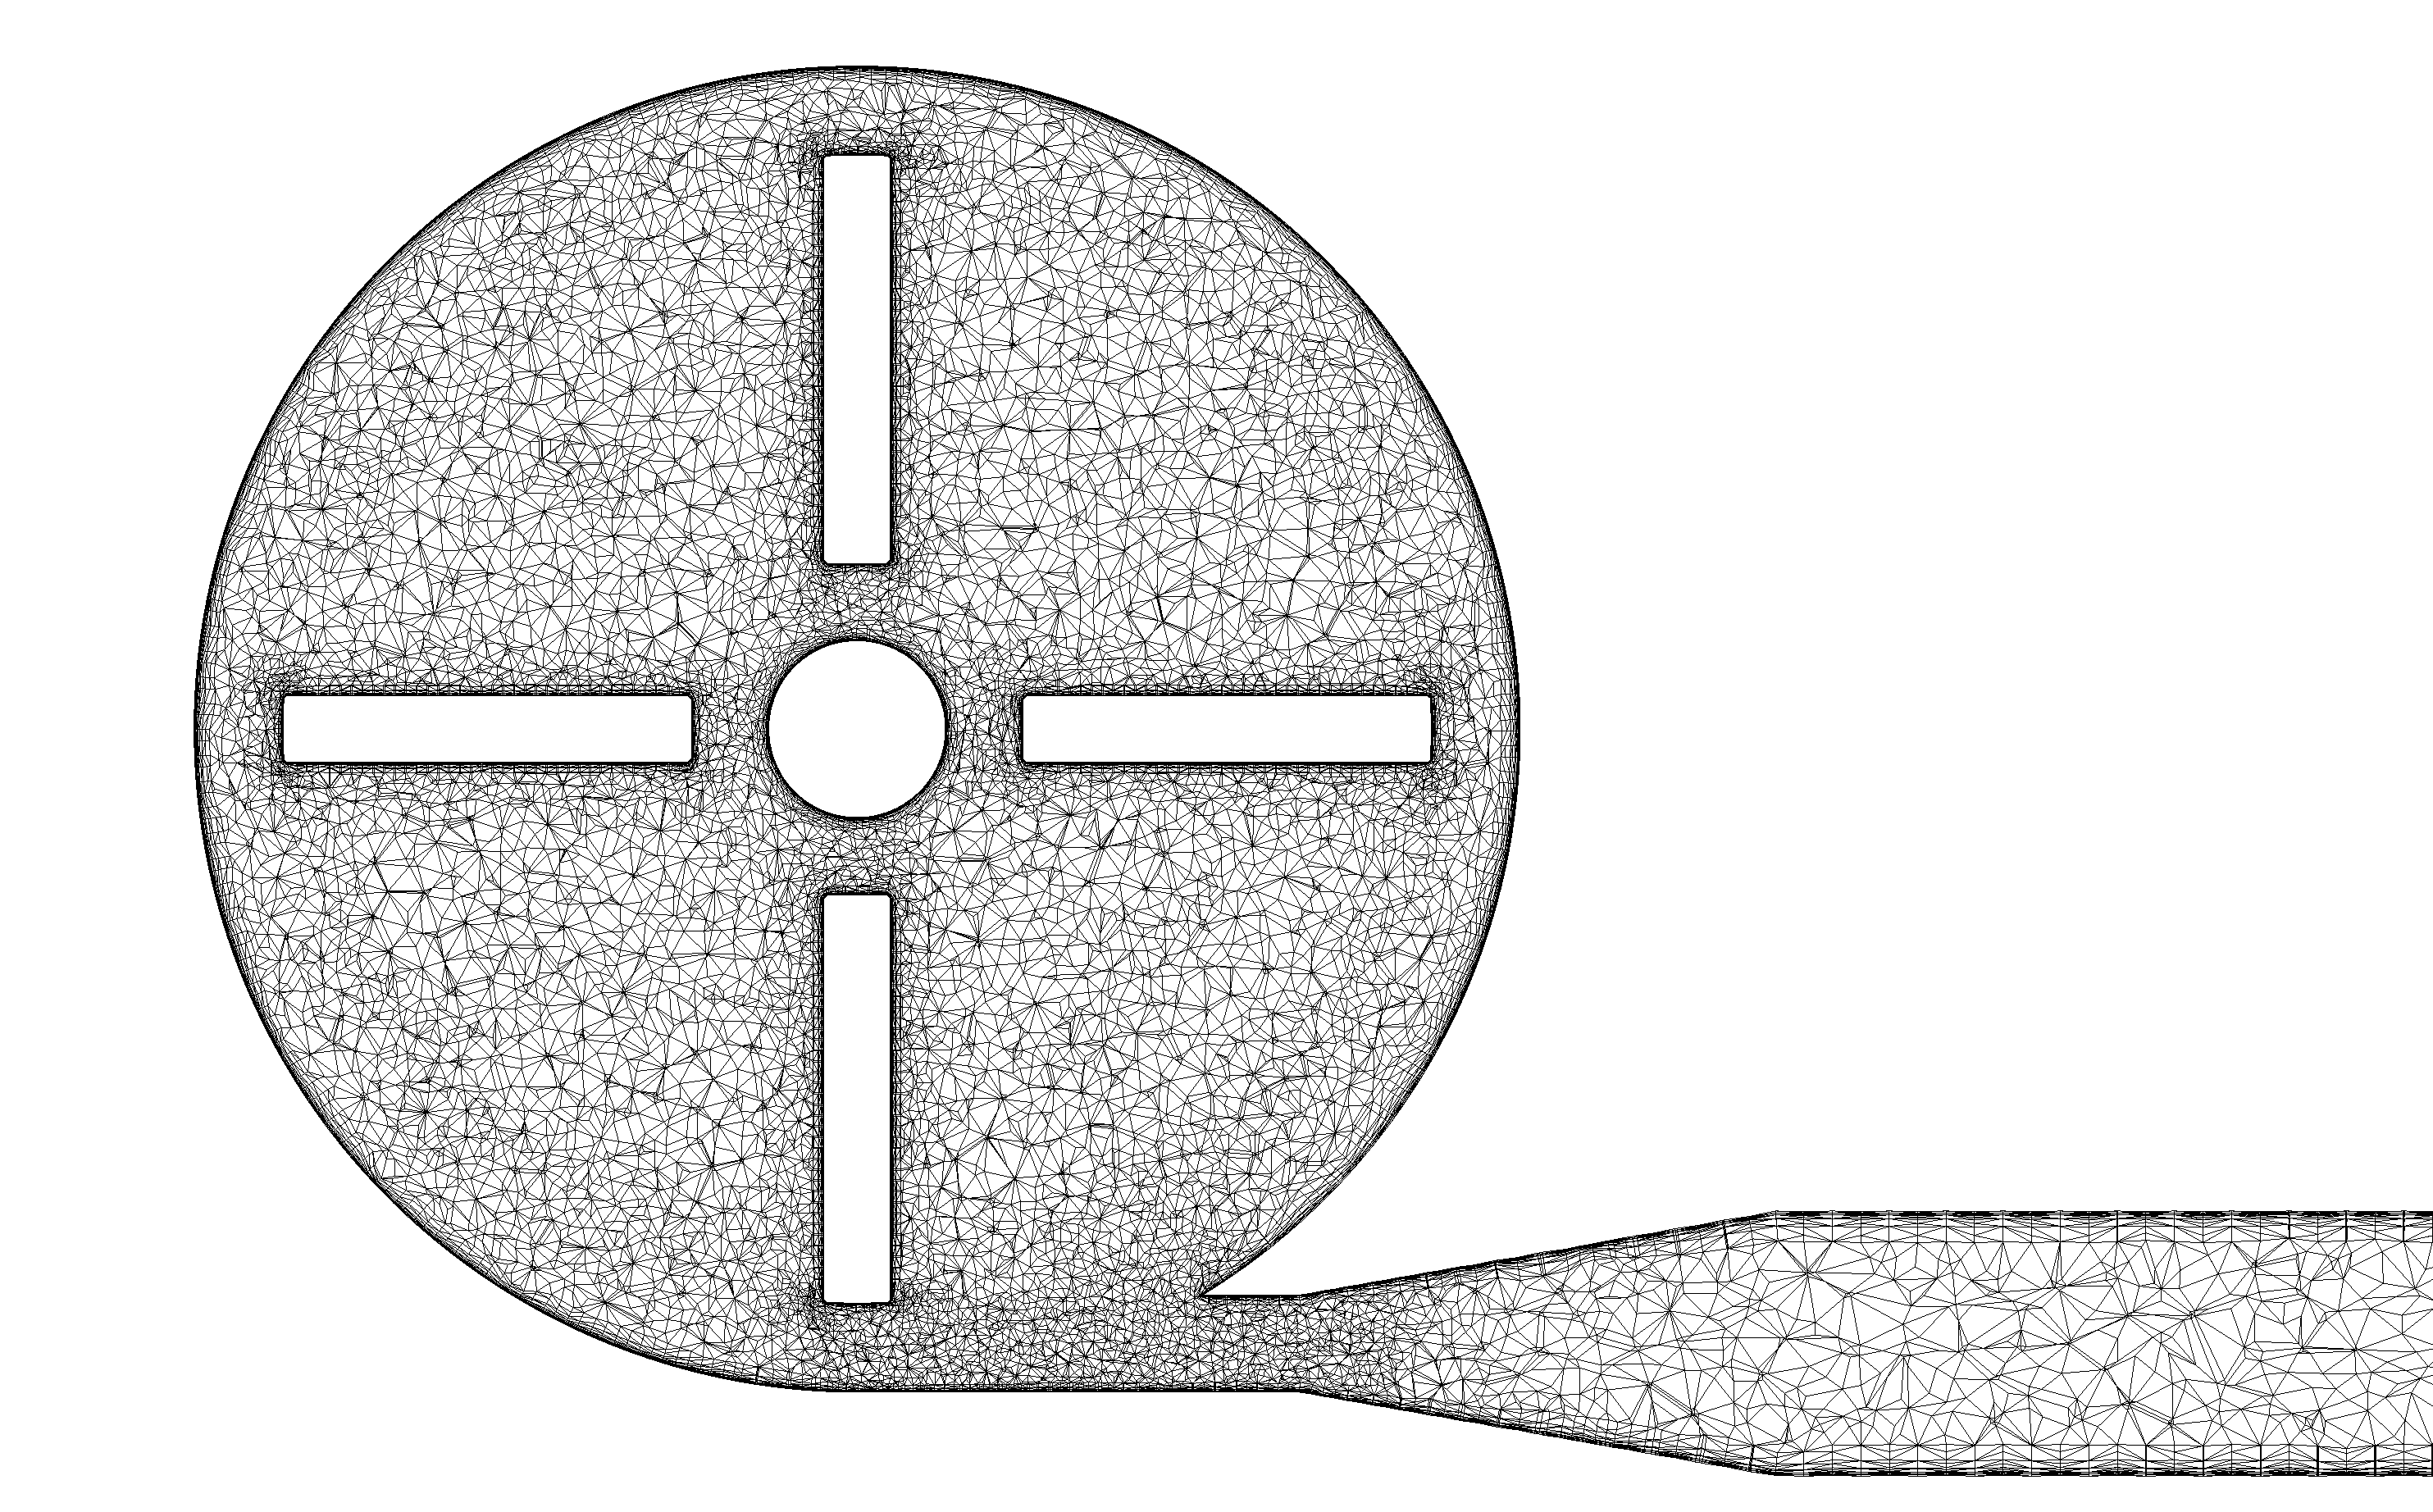
\includegraphics[width=3in]{imgs/nozzle_pump/pump_mesh_2.pdf}
    \caption{The mesh configuration used in the pump flow simulations on the plane coinciding with the mid-axis plane of the outlet diffuser.}
    \label{fig:pumpmesh}
\end{figure}

% pump result & analysis
The pressure difference across the pump obtained by the experiment and the simulations are listed in Table~\ref{tab:pumppres}. Using FEM the discrepancy with experiment is only $3.6$\%. On the other hand, PFEM-2 predicts a lower pressure difference with $14.6$\% discrepancy compared to the experiment. From the distribution of the velocity and pressure fields in the chamber (Fig. \ref{fig:pumpvel} and \ref{fig:pumppres}, the results by PFEM-2 and FEM are qualitatively in accordance with each other. Some discrepancies of the velocity field can be found at the trailing edge near the blade tips, and in the jet flow in the diffuser. 

%it can be observed that the velocity pattern obtained with PFEM-2 is different from FEM. With PFEM-2, the velocity is higher mainly in front of the leading edge of the blade, where with FEM, the velocity is higher at both side of the blade, but more on the trailing edge. \textbf{CHECK:} ***This might be due to in the present PFEM-2 method, the advection and viscous effect are treated separately and sequentially, and an explicit integration scheme is employed. As a result, the particles pushed by the rotor blades have less tendency to turn in chamber than FEM, which can be observed from the streamline plot in Fig.~\ref{fig:pumpsl}. This leads to a larger pressure gradient in the radial direction in order to make particles turn in the chamber. ***

\begin{table}[h]
\caption {Pressure differences across the pump.}\label{tab:pumppres} 
\centering
\begin{tabular}{|c|c|}
\hline
 & Pressure (mmHg) \\ \hline
Experiment \cite{mali_cfd}    & 272.38    \\ \hline
FEM    & 282.40             \\ \hline
PFEM-2    & 232.59          \\ \hline
\end{tabular}
\end{table}

\begin{figure}[htbp]
    \centering
    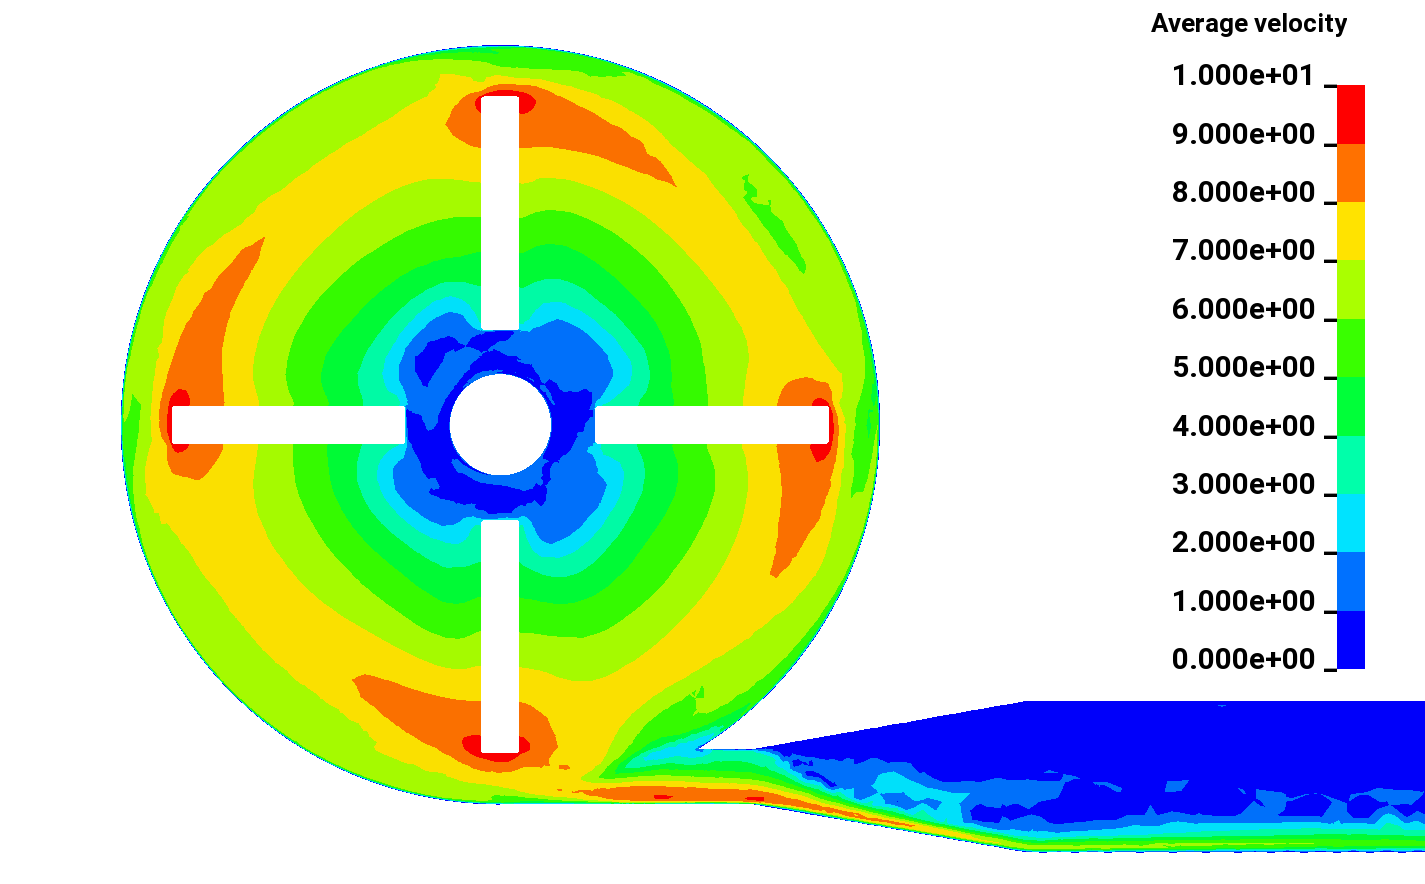
\includegraphics[width=3in]{imgs/nozzle_pump/pumpvel_fem.png}\\
    \vspace{.5cm}
    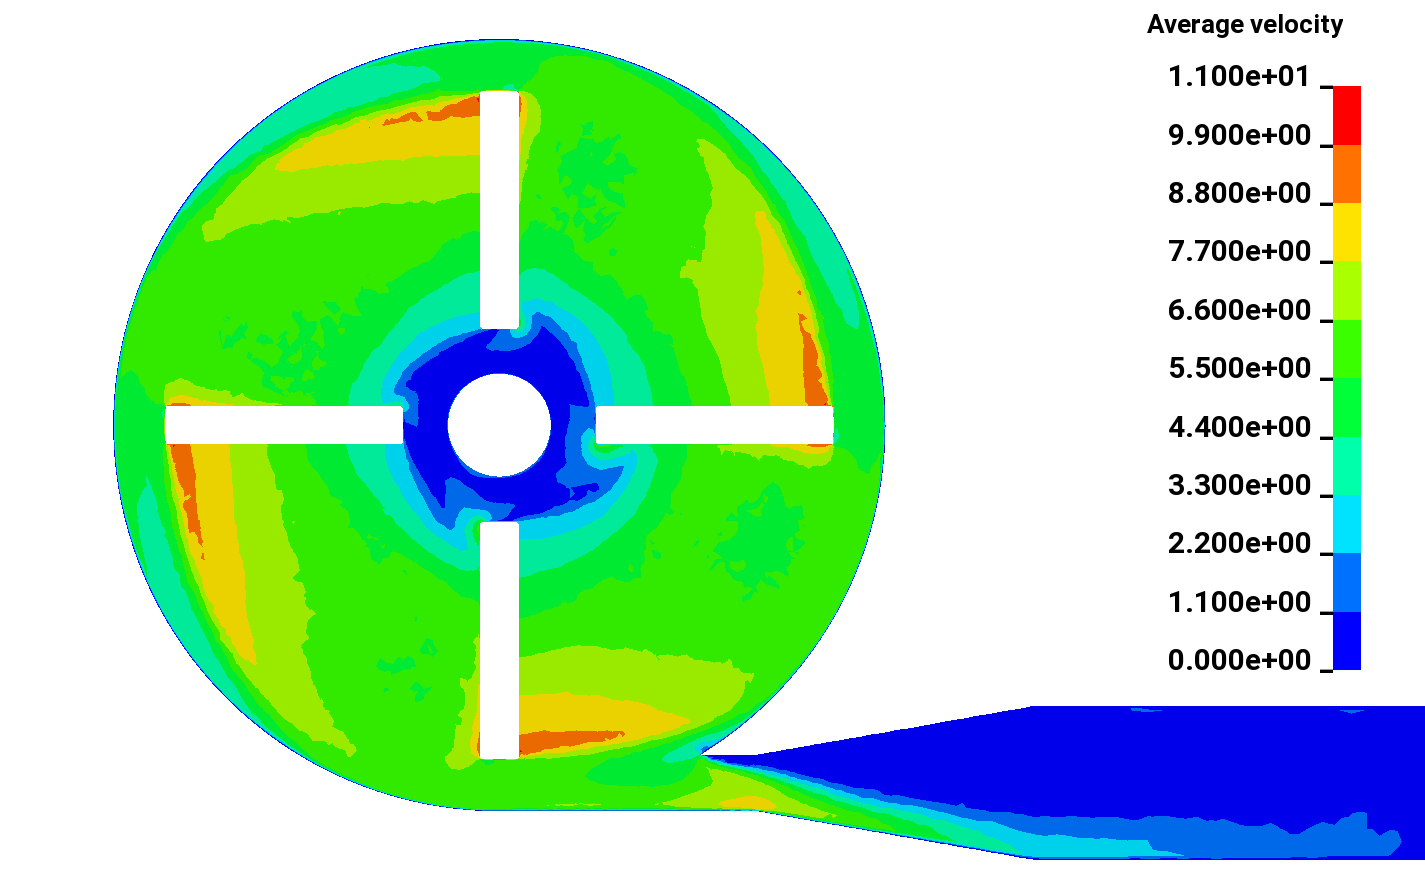
\includegraphics[width=3in]{imgs/nozzle_pump/pumpvel_pfem.png}
    \caption{The velocity magnitude distribution on the plane which coincides to the mid-axis plane of the outlet diffuser using FEM (top) and PFEM-2 (bottom).}
    \label{fig:pumpvel}
\end{figure}

\begin{figure}[htbp]
    \centering
    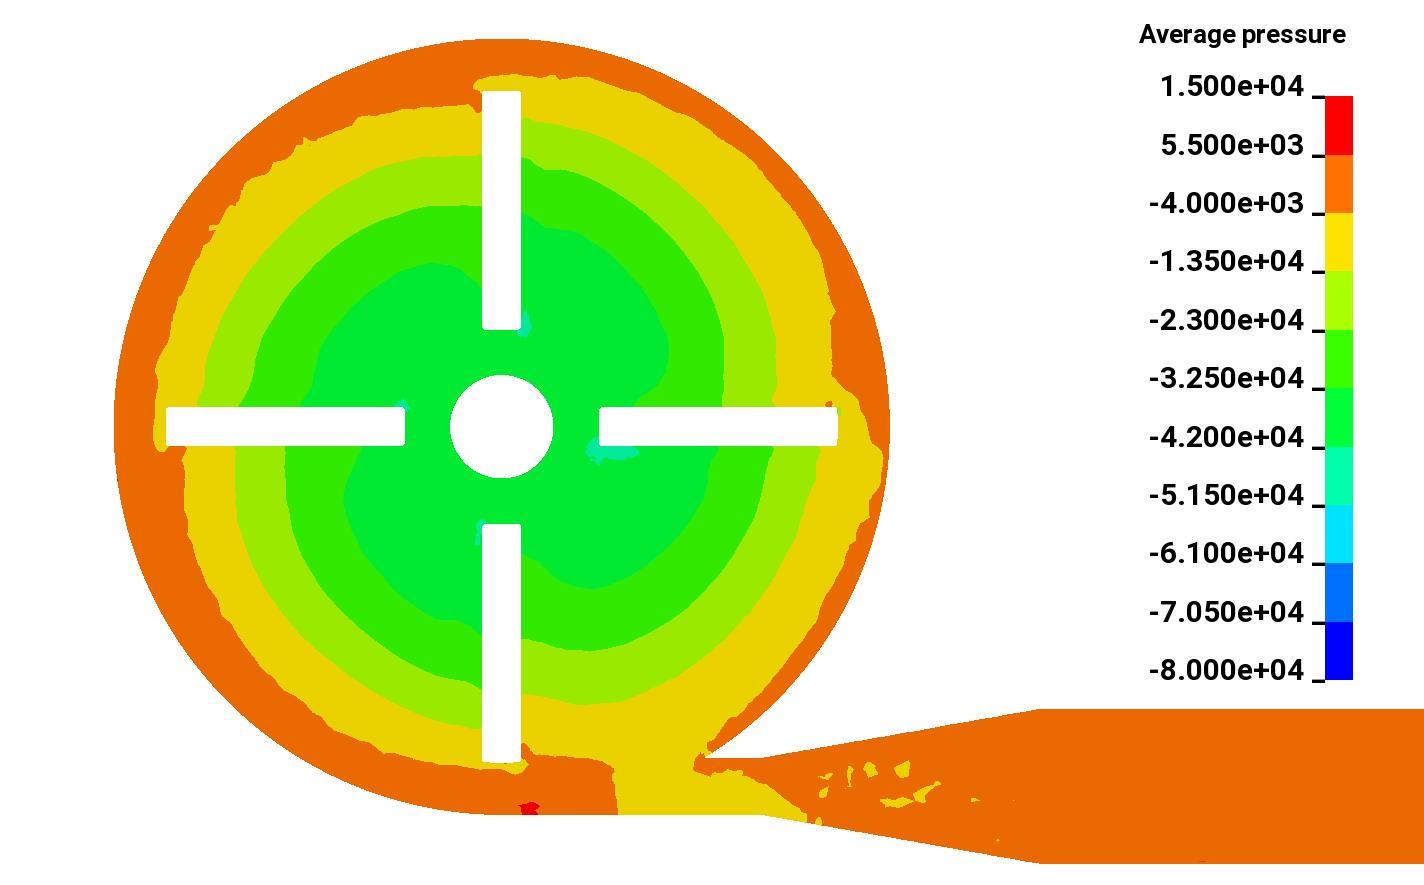
\includegraphics[width=3in]{imgs/nozzle_pump/pumppres_fem.png}\\
    \vspace{.5cm}
    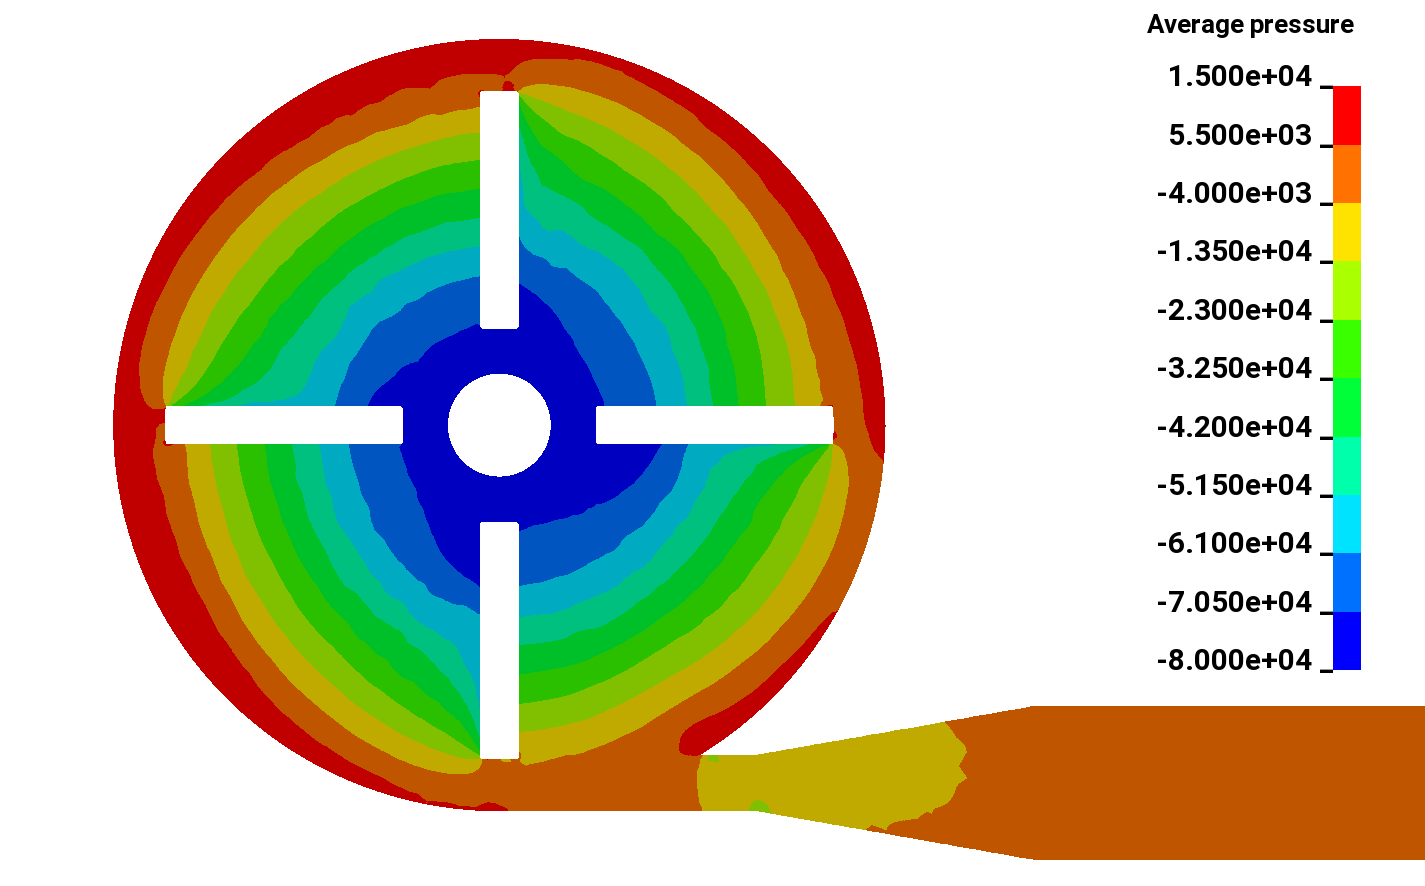
\includegraphics[width=3in]{imgs/nozzle_pump/pumppres_pfem.png}
    \caption{The pressure distribution on the plane which coincides to the mid-axis plane of the outlet diffuser using FEM (top) and PFEM-2 (bottom).}
    \label{fig:pumppres}
\end{figure}

Fig.~\ref{fig:pumpvelprofile} depicts the comparison of the velocity profile in the pump chamber and diffuser compared with the experimental measurements \cite{mali_cfd}. The velocity profile between blades by FEM and PFEM-2 are both in accordance with experiments. In the outlet diffuser, FEM predicts the detached jet leaning more against the outer wall and the velocity magnitude appears to be larger than experiments. The phenomenon may be due to the usage of the non-inertial reference frame approximation since similar velocity distribution in the diffuser can also be observed in most of the other numerical results that use non-inertial reference frame \cite{mali_cfd}.  
 
\begin{figure}[htbp]
    \centering
    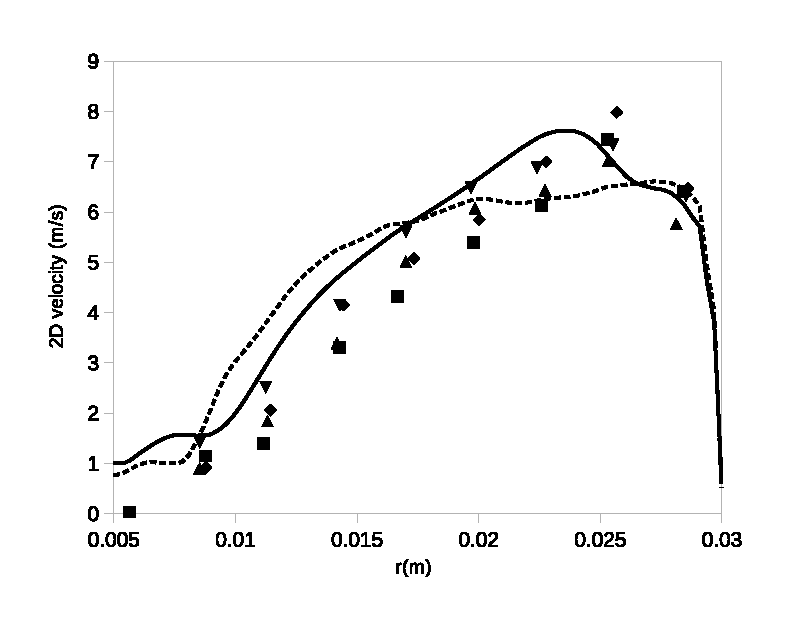
\includegraphics[width=3in]{imgs/nozzle_pump/pump_velblade.eps}\\
    \vspace{.5cm}
    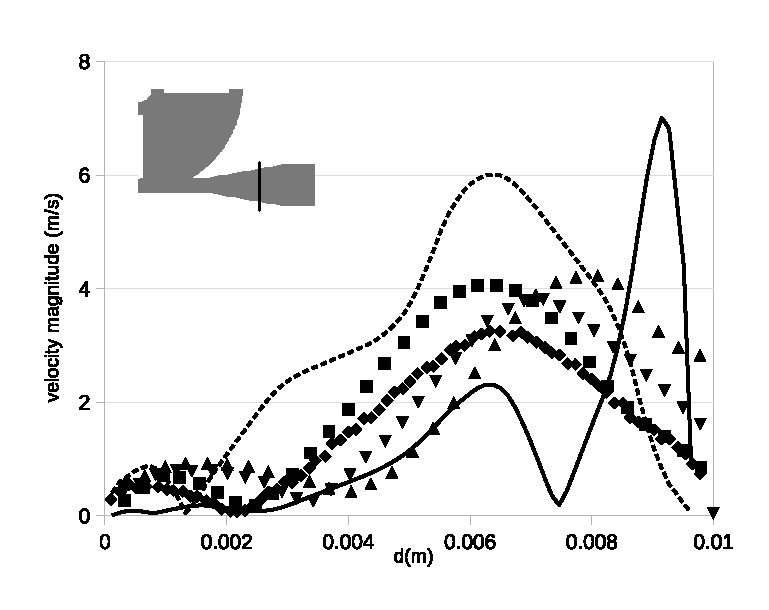
\includegraphics[width=3in]{imgs/nozzle_pump/pump_veldiffuser.eps}
    \caption{The magnitude of the two-dimensional velocity on the same plane as in Figs.~\ref{fig:pumpvel} and \ref{fig:pumppres} with experiments and simulations. Top: velocity profile between two blades where $r$ refers to the radius to rotor center. Right: across the outlet diffuser where $d$ refers to distance to the inner wall. $\blacktriangledown$ $\blacktriangle$ $\blacksquare$ $\blacklozenge$: experiments \cite{mali_cfd}. Solid line: FEM. Dashed line: PFEM-2. }
    \label{fig:pumpvelprofile}
\end{figure}

\subsection{Vena Cava}

\subsubsection*{Grid Convergence Test}

The simulations of the flow in Vena Cava are conducted according to the parameters provided in \cite{craven_cfd}. The simulations of two flowrates are performed corresponding to the rest and exercise conditions. The density is $\rho=1817$, $\nu=3.21\times10^{-6}$ (rest) and $\nu=3.02\times10^{-6}$(exercise), and flowrate $Q= 0.5$ (l/min) and $3$ (l/min) into two iliac veins separately. The corresponding Reynolds numbers for rest and exercise conditions are 236 and 1505. The flow is considered to be laminar in the Vena Cava.
For boundary conditions, the parabolic velocity profile is prescribed at the inlet of two iliac veins. And the zero pressure condition is imposed at the outlet of the Vena Cava. 

For the mesh convergence test, 4 kinds of mesh sizes are used in the test. The mesh size and the total number of tetrahedral element for these 4 meshes are listed in the Table 1. The transverse cross-sections of all 4 meshes, which are located at 10 cm downstream of the after the merging location of two iliac veins, are shown in the Figure 1.

\begin{table}[h]
\caption {Mesh used in the convergence test.} \label{tab:meshsize}
\centering
\begin{tabular}{|c|c|c|}
\hline
Mesh & Number of element ($\times10^6$)& mesh size (mm) \\ \hline
1    & 0.87              & 2.0              \\ \hline
2    & 2.04              & 1.4            \\ \hline
3    & 4.70              & 1.0               \\ \hline
4    & 17.68             & 0.6            \\ \hline
5    & 37.94             & 0.45            \\ \hline
\end{tabular}
\end{table}


\begin{figure*}[htbp]
    \centering
    \begin{minipage}[c][2in][c]{0.4\linewidth}
        \centering
        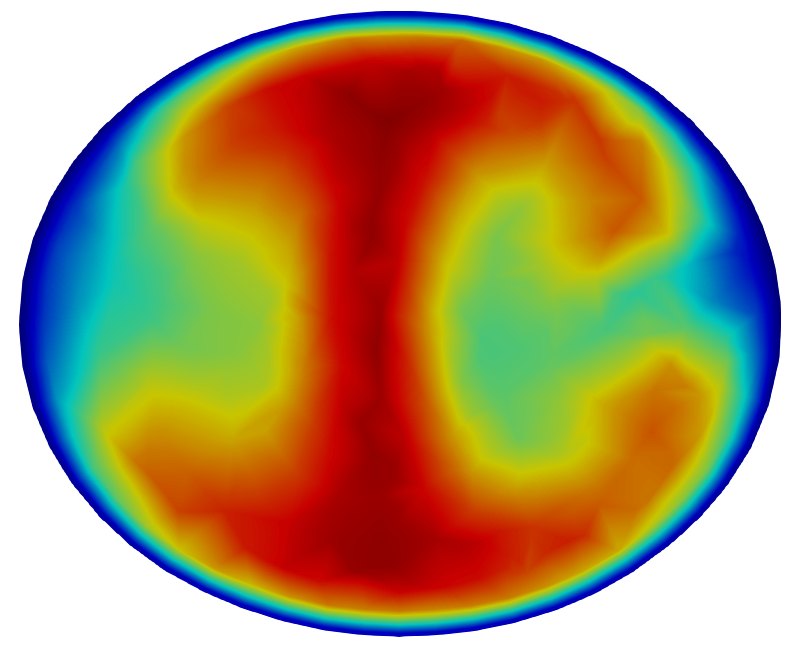
\includegraphics[width=2.3in]{imgs/vena_cava/Umag_mesh1.png}\\
        mesh 1
    \end{minipage}
    \begin{minipage}[c][2in][c]{0.4\linewidth}
        \centering
        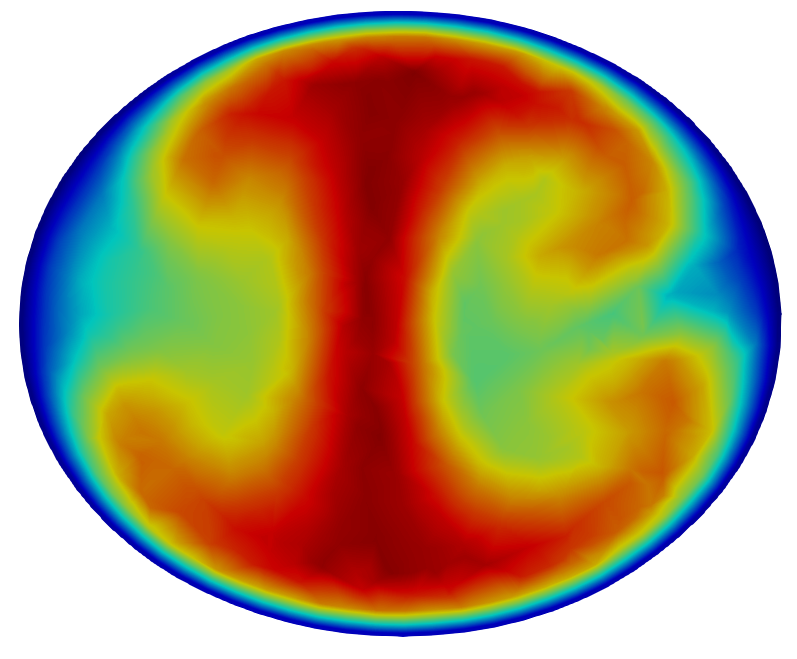
\includegraphics[width=2.3in]{imgs/vena_cava/Umag_mesh2.png}\\
        mesh 2
    \end{minipage}\\[.5\baselineskip]
    \begin{minipage}[c][2in][c]{0.4\linewidth}
        \centering
        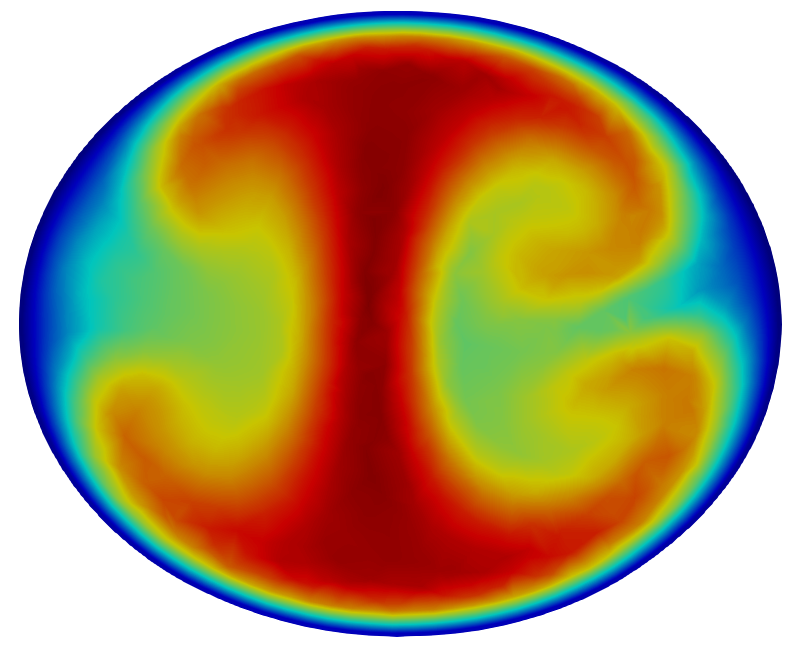
\includegraphics[width=2.3in]{imgs/vena_cava/Umag_mesh3.png}\\
        mesh 3
    \end{minipage}
    \begin{minipage}[c][2in][c]{0.4\linewidth}
        \centering
        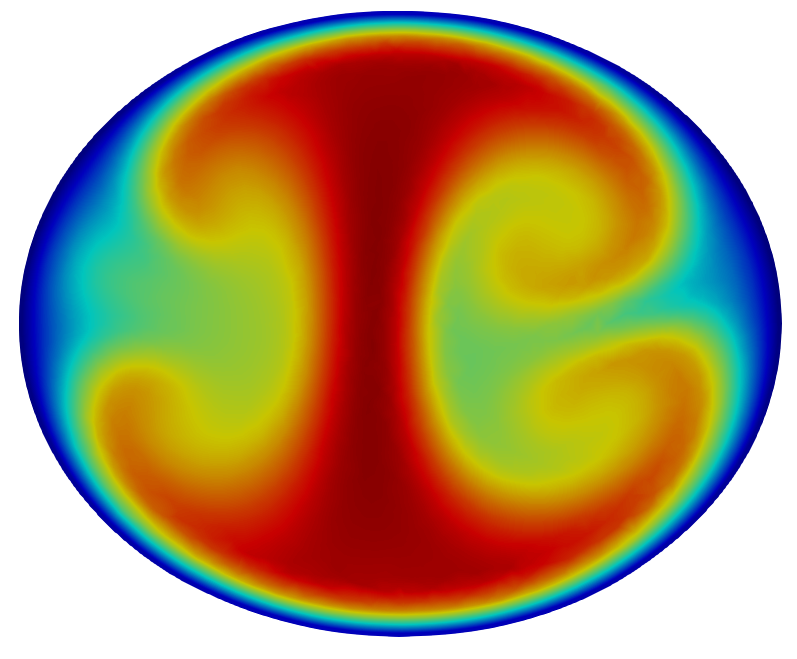
\includegraphics[width=2.3in]{imgs/vena_cava/Umag_mesh4.png}\\
        mesh 4
    \end{minipage}\\[.5\baselineskip]
    \begin{minipage}[c][2in][c]{0.4\linewidth}
        \centering
        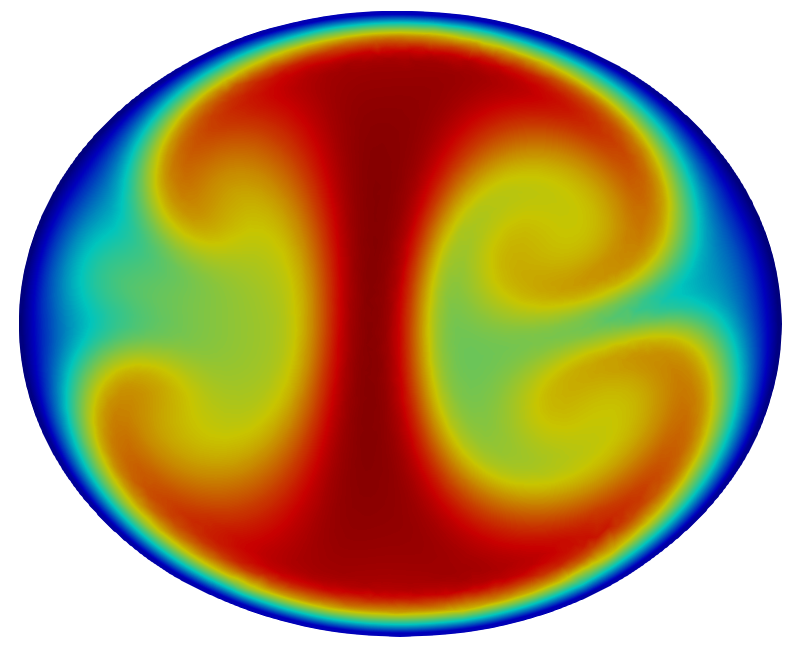
\includegraphics[width=2.3in]{imgs/vena_cava/Umag_mesh5.png}\\
        mesh 5
    \end{minipage}
    \begin{minipage}[c][2in][c]{0.4\linewidth}
        \centering
        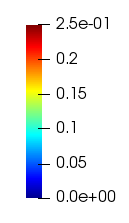
\includegraphics[width=.7in]{imgs/vena_cava/colormap_exercise.png}\\
    \end{minipage}
    \caption{The velocity magnitude fields using different sizes of mesh.}
    \label{fig:velmag}
\end{figure*}

\begin{figure*}[htbp]
    \centering
    \begin{minipage}[c][2in][c]{0.4\linewidth}
        \centering
        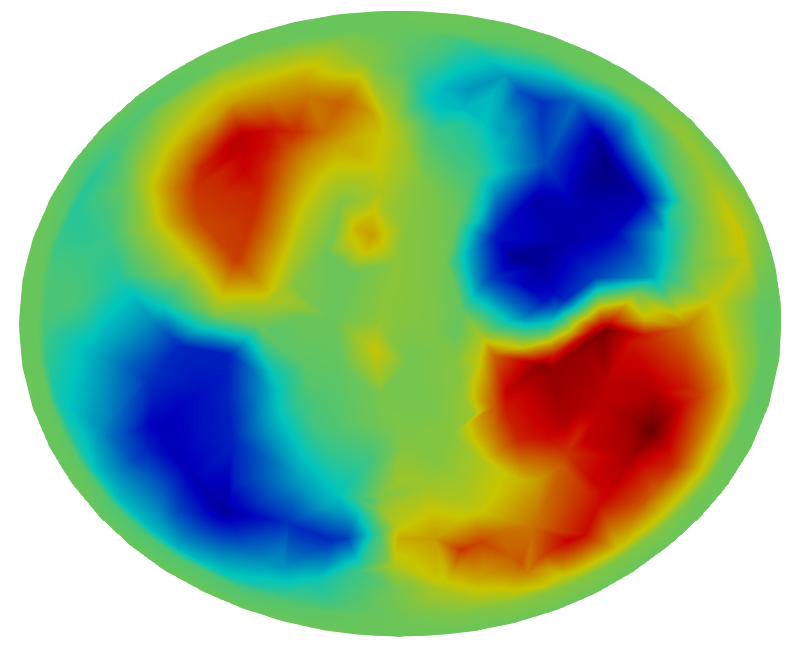
\includegraphics[width=2.3in]{imgs/vena_cava/LNH_mesh1.png}\\
        mesh 1
    \end{minipage}
    \begin{minipage}[c][2in][c]{0.4\linewidth}
        \centering
        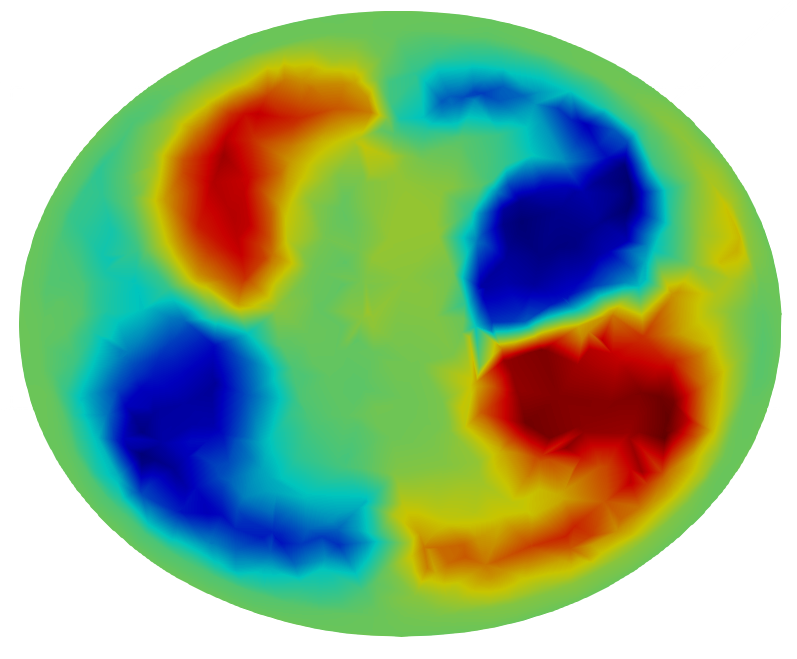
\includegraphics[width=2.3in]{imgs/vena_cava/LNH_mesh2.png}\\
        mesh 2
    \end{minipage}\\[.5\baselineskip]
    \begin{minipage}[c][2in][c]{0.4\linewidth}
        \centering
        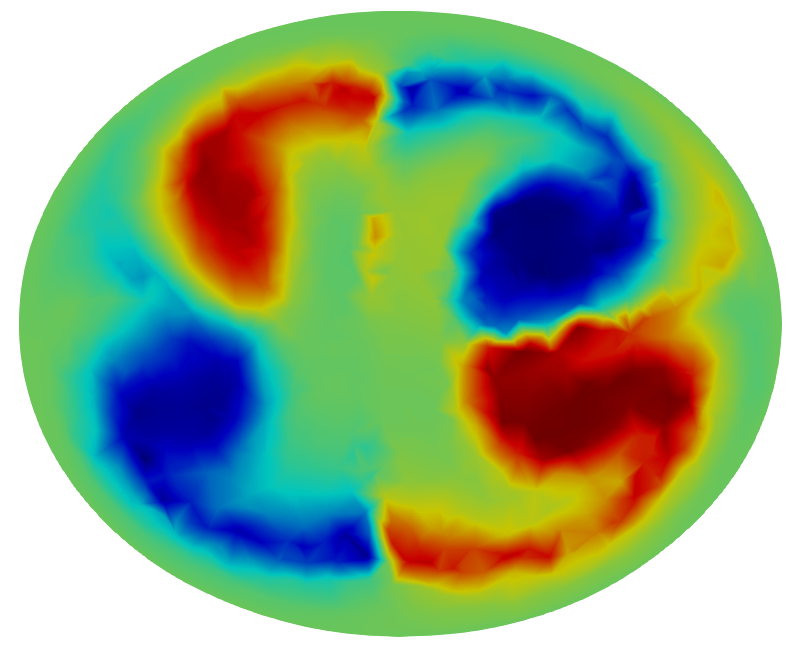
\includegraphics[width=2.3in]{imgs/vena_cava/LNH_mesh3.png}\\
        mesh 3
    \end{minipage}
    \begin{minipage}[c][2in][c]{0.4\linewidth}
        \centering
        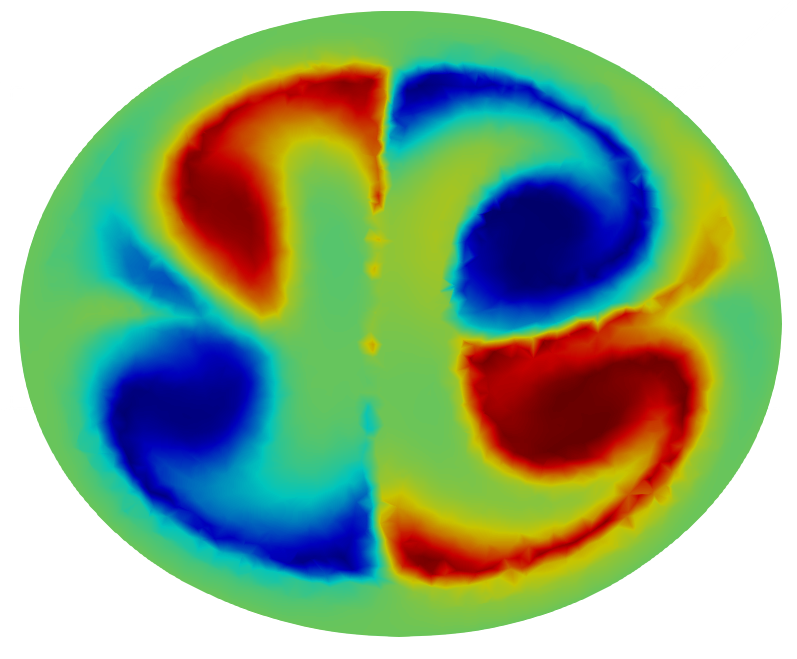
\includegraphics[width=2.3in]{imgs/vena_cava/LNH_mesh4.png}\\
        mesh 4
    \end{minipage}\\[.5\baselineskip]
    \begin{minipage}[c][2in][c]{0.4\linewidth}
        \centering
        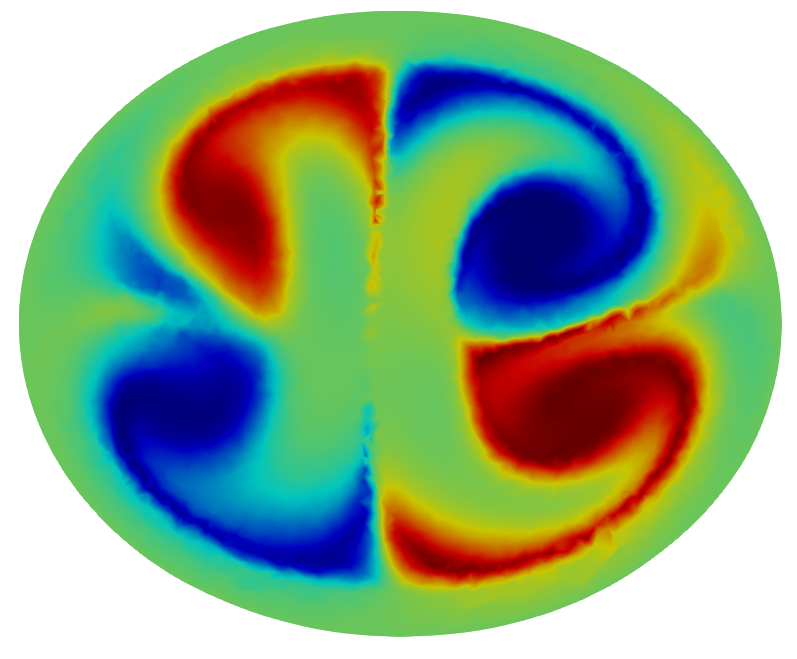
\includegraphics[width=2.3in]{imgs/vena_cava/LNH_mesh5.png}\\
        mesh 5
    \end{minipage}
    \begin{minipage}[c][2in][c]{0.4\linewidth}
        \centering
        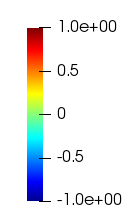
\includegraphics[width=.7in]{imgs/vena_cava/colormap_LNH.png}\\
    \end{minipage}
    \caption{The local normalized helicity (LNH) fields.}
    \label{fig:lnh}
\end{figure*}

% choose either one: with  p or not with p
\begin{table*}[]
\centering
\caption {Value of maximum velocity, transverse velocity, Helicity and the correspoding convergence rates.} \label{tab:convergence}
\begin{tabular}{|c|c|c|c|c|c|c|}
\hline
     & \multicolumn{2}{c|}{maximum velocity} & \multicolumn{2}{c|}{transverse velocity} & \multicolumn{2}{c|}{Helicity} \\ \hline
Mesh & $\left |u\right |_{max} $    & p             & $\overline{\left |u\right |}_{tr}$          & p              &   $\overline{HI}$              & p           \\ \hline
1    & 0.2549               &               & 0.0238                 &                & 0.3807         &             \\ \hline
2    & 0.2585               &               & 0.0244                 &                & 0.4132         &             \\ \hline
3    & 0.2567               & 2.36       & 0.0247                 & 2.40          & 0.4331         & 1.63        \\ \hline
4    & 0.2541               & 0.31       & 0.02497                 & 2.24          & 0.4498         & 1.84        \\ \hline
5    & 0.2534	          &  2.16      & 0.02502                 & 2.88          & 0.4536         &  2.54        \\ \hline
\end{tabular}
\end{table*}
% 
\iffalse
\begin{table}[h]
\caption {} \label{tab:convergence}
\centering
\begin{tabular}{|c|c|c|c|}
\hline
Mesh & $u_{max}$ & Transverse velocity &  Helicity       \\ \hline
1    & 0.25486           & 0.02380        & 0.38067 \\ \hline
2    & 0.25846           & 0.02443        & 0.41316 \\ \hline
3    & 0.25666           & 0.02474        & 0.43313 \\ \hline
4    & 0.25409           & 0.02497        & 0.44978 \\ \hline
5     & 0.25341	      & 0.02502        & 0.45361         \\ \hline
\end{tabular}
\end{table}
\fi
%------------------------------------

\subsubsection*{Comparison with Experimental Results}

\begin{figure*}\centering
\begin{minipage}[c][10cm][c]{0.25\textwidth}
\centering
\vspace*{\fill}
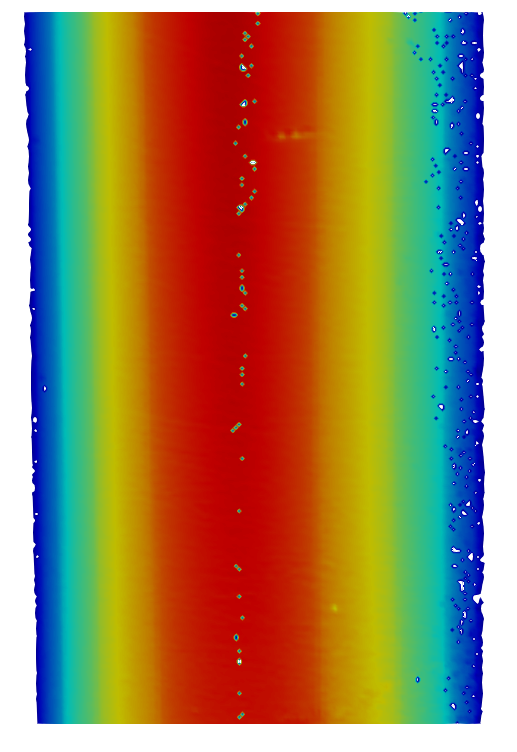
\includegraphics[height=4cm]{imgs/vena_cava/PIV_coronal_rest.png}
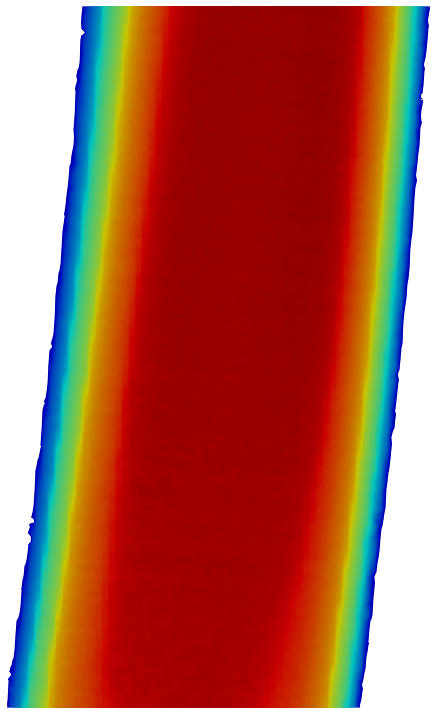
\includegraphics[height=5cm]{imgs/vena_cava/PIV_sagittal_rest.png}
\\PIV
\end{minipage}
\begin{minipage}[c][10cm][c]{0.25\textwidth}
\centering
\vspace*{\fill}
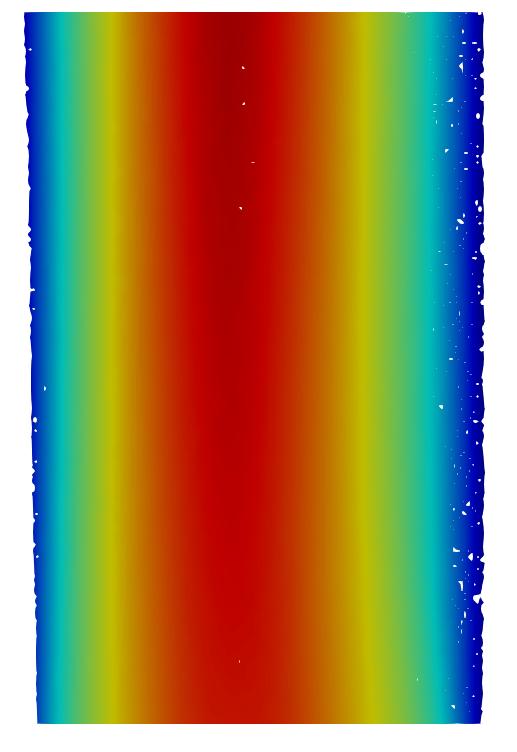
\includegraphics[height=4cm]{imgs/vena_cava/FEM_coronal_rest.png}
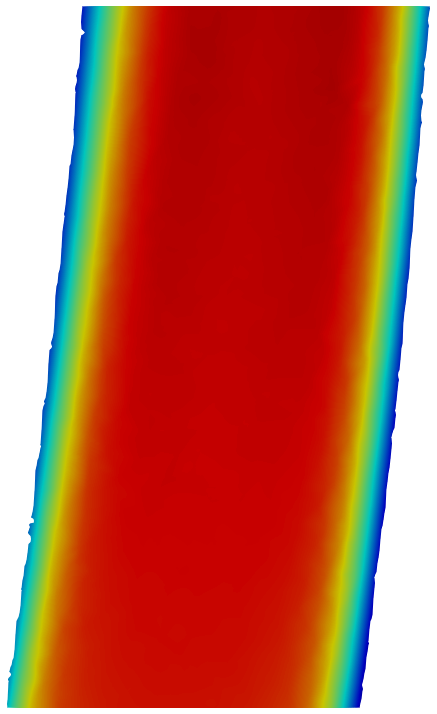
\includegraphics[height=5cm]{imgs/vena_cava/FEM_sagittal_rest.png}
\\FEM
\end{minipage}
\begin{minipage}[c][10cm][c]{0.25\textwidth}
\centering
\vspace*{\fill}
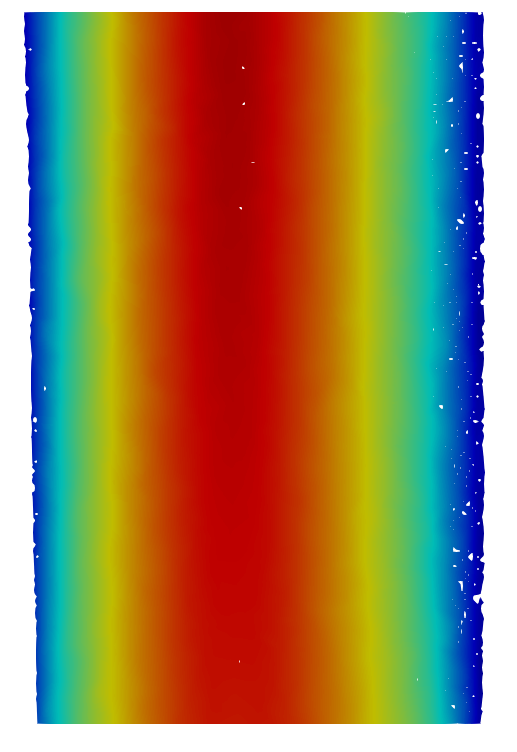
\includegraphics[height=4cm]{imgs/vena_cava/PFEM_coronal_rest.png}
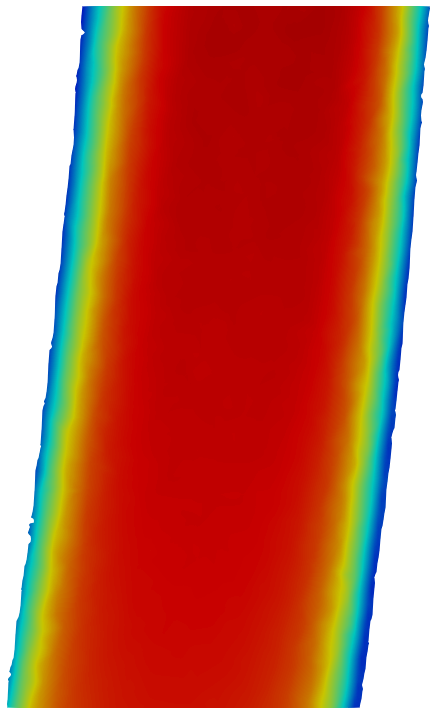
\includegraphics[height=5cm]{imgs/vena_cava/PFEM_sagittal_rest.png}
\\PFEM-2
\end{minipage}
\begin{minipage}[c][10cm][t]{0.1\textwidth}
\vspace*{\fill}
\centering
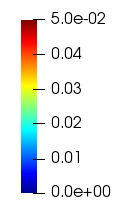
\includegraphics[height=3cm]{imgs/vena_cava/colormap_rest.png}
\\
\end{minipage}
\caption{The in-plane 2D velocity magnitude in coronal (top) and sagittal (bottom) planes of PIV, FEM and PFEM-2 results at resting condition}
\label{fig:process1}
\end{figure*}

\begin{figure*}\centering
\begin{minipage}[c][10cm][c]{0.25\textwidth}
\centering
\vspace*{\fill}
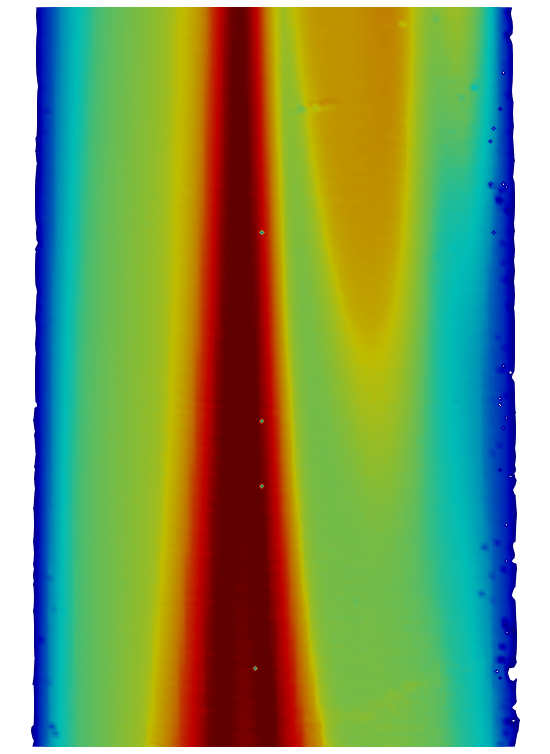
\includegraphics[height=4cm]{imgs/vena_cava/PIV_coronal_exercise.png}
\includegraphics[height=5cm]{imgs/vena_cava/PIV_sagittal_exercise.png}
\\PIV
\end{minipage}
\begin{minipage}[c][10cm][c]{0.25\textwidth}
\centering
\vspace*{\fill}
\includegraphics[height=4cm]{imgs/vena_cava/FEM_coronal_exercise.png}
\includegraphics[height=5cm]{imgs/vena_cava/FEM_sagittal_exercise.png}
\\FEM
\end{minipage}
\begin{minipage}[c][10cm][c]{0.25\textwidth}
\centering
\vspace*{\fill}
\includegraphics[height=4cm]{imgs/vena_cava/PFEM_coronal_exercise.png}
\includegraphics[height=5cm]{imgs/vena_cava/PFEM_sagittal_exercise.png}
\\PFEM-2
\end{minipage}
\begin{minipage}[c][10cm][t]{0.1\textwidth}
\vspace*{\fill}
\centering
\includegraphics[height=3cm]{imgs/vena_cava/colormap_exercise.png}
\\
\end{minipage}
\caption{The in-plane 2D velocity magnitude in coronal (top) and sagittal (bottom) planes of PIV, FEM and PFEM-2 results at resting condition}
\label{fig:process1}
\end{figure*}

\begin{table}[h!]
\caption {Global relative error (\%) between CFD and PIV at resting condition} \label{tab:convergence}
\centering
\begin{tabular}{|c|c|c|}
\hline
       & Coronal & Sagittal \\ \hline
CFD from \cite{craven_cfd}  & 3.07    & 6.77     \\ \hline
FEM    & 4.83    & 6.62     \\ \hline
PFEM-2 & 4.79    & 6.65     \\ \hline
\end{tabular}
\end{table}

\begin{table}[h!]
\caption {Global relative error (\%) between CFD and PIV at exercising condition} \label{tab:convergence}
\centering
\begin{tabular}{|c|c|c|}
\hline
       & Coronal & Sagittal \\ \hline
CFD from \cite{craven_cfd}  & 10.98	&5.56 \\ \hline
FEM    &  11.28    &  5.93  \\ \hline
PFEM-2 &  10.44   &  6.10     \\ \hline
\end{tabular}
\end{table}


\section{Conclusions}

%\clearpage
\begin{thebibliography}{9}
  \bibitem{cpi1} FDA’s ``Critical Path'' Computational Fluid Dynamics (CFD)/Blood Damage Project: Computational Round Robin problems
https://nciphub.org/wiki/FDA\_CFD
\bibitem{cpi} FDA Critical Path Initiative (CPI) \\\small{https://www.fda.gov/scienceresearch/specialtopics/criticalpathinitiative/default.htm}
\bibitem{fda_res} Hariharan, P., Giarra, M., Reddy, V., Day, S.W.,
Manning, K.B., Deutsch, S., Stewart, S.F., Myers, M.R., Berman, M.R., Burgreen, G.W. and Paterson, E.G. (2011).
Multilaboratory particle image velocimetry analysis of the FDA benchmark nozzle model to support validation of computational
fluid dynamics simulations. Journal of Biomechanical Engineering, 133(4), 041002.
\bibitem{fda_nozzle} Herbertson, L. H., Olia, S. E., Daly, A., Noatch, C. P., Smith, W. A., Kameneva, M. V., \& Malinauskas, R. A. (2015).
Multilaboratory Study of Flow‐Induced Hemolysis Using the FDA Benchmark Nozzle Model. Artificial organs, 39(3), 237-248.
\bibitem{fda_pump} Giarra, M. N. (2009). Shear Stress Distribution and Hemolysis Measurements in a Centrifugal Blood Pump. Rochester Institute of
Technology.
\bibitem{fda_numrob} Zmijanovic, V., Mendez, S., Moureau, V., \& Nicoud, F. (2017). About the numerical robustness of biomedical benchmark cases:
Interlaboratory FDA's idealized medical device. International journal for numerical methods in biomedical engineering, 33(1).
\bibitem{hariharan_nozzle} Hariharan, P., D’Souza, G. A., Horner, M., Morrison, T. M., Malinauskas, R. A., \& Myers, M. R. (2017). Use of the FDA nozzle
model to illustrate validation techniques in computational fluid dynamics (CFD) simulations. PloS one, 12(6), e0178749.
\bibitem{nassau_pump} Nassau, C. J., Wray, T. J., \& Agarwal, R. K. (2015, July). Computational Fluid Dynamic Analysis of a Blood Pump: An FDA
Critical Path Initiative. In ASME/JSME/KSME 2015 Joint Fluids Engineering Conference (pp. V002T26A002-V002T26A002).
American Society of Mechanical Engineers.
\bibitem{heck_hemo} Heck, M. L., Yen, A., Snyder, T. A., O'Rear, E. A., \& Papavassiliou, D. V. (2017). Flow‐Field Simulations and Hemolysis
Estimates for the Food and Drug Administration Critical Path Initiative Centrifugal Blood Pump. Artificial organs, 41(10).
\bibitem{stewart_cfd} Stewart, S. F., Paterson, E. G., Burgreen, G. W., Hariharan, P., Giarra, M., Reddy, V., Stewart, S.F., Paterson, E.G., Burgreen,
G.W., Hariharan, P., Giarra, M., Reddy, V., Day, S.W., Manning, K.B., Deutsch, S., Berman, M.R. and Myers, M.R. (2012).
Assessment of CFD performance in simulations of an idealized medical device: results of FDA’s first computational
interlaboratory study. Cardiovascular Engineering and Technology, 3(2), 139-160.
\bibitem{mali_cfd} Malinauskas, R. A., Hariharan, P., Day, S. W., Herbertson, L. H., Buesen, M., Steinseifer, U., Aycock, K.I., Good, B.C., Deutsch,
S., Manning, K.B. and Craven, B.A. (2017). FDA benchmark medical device flow models for CFD validation. ASAIO Journal,
63(2), 150-160.
\bibitem{gallagher_exp} Gallagher, M.B., Aycock, K.I., Craven, B.A. et al. Cardiovasc Eng Tech (2018) 9: 641. https://doi.org/10.1007/s13239-018-00390-2
\bibitem{craven_cfd} Craven, B.A., Aycock, K.I. \& Manning, K.B. Cardiovasc Eng Tech (2018) 9: 654. https://doi.org/10.1007/s13239-018-00392-0
\bibitem{sph} Monaghan JJ (1988) An introduction to SPH. Comput Phys Com-
mun 48:89–96
\bibitem{pic} Harlow FH (1955) A machine calculation method for hydro-
dynamic problems. Los Alamos Scientific Laboratory Report
LAMS-1956
\bibitem{mac} Harlow FH, Welch J (1965) Numerical calculation of time depen-
dent viscous incompressible flow of fluid with free surface. Phys
Fluids 8(12):2182–2189
\bibitem{mpm} Wieckowsky Z (2004) The material point method in large
strain engineering problems. Comput Methods Appl Mech Eng
193(39):4417–4438
\bibitem{sergio:pfem} Idelsohn SR, Oñate E, Del Pin F (2004) The particle finite element
method a powerful tool to solve incompressible flows with free-
surfaces and breaking waves. Int J Numer Methods 61:964–989

\bibitem{sergio:xivs1} Idelsohn SR, Nigro NM, Limache A, Oñate E (2012) Large
time-step explicit integration method for solving problems with
dominant convection. Comput Methods Appl Mech Eng 217–
220:168–185

\bibitem{sergio:xivs2} Idelsohn SR, Nigro NM, Gimenez JM, Rossi R, Marti J (2013)
A fast and accurate method to solve the incompressible Navier–
Stokes equations. Eng Comput 30(2):197–222

\bibitem{gimenez:parallel} Gimenez JM, Nigro NM, Idelsohn SR (2014) Evaluating the perfor-
mance of the particle finite element method in parallel architectures.
J Comput Part Mech 1(1):103–116

\bibitem{sergio:pfem2_lts} Idelsohn SR, Marti J, Becker P, Oñate E (2014) Analysis of mul-
tifluid flows with large time steps using the particle finite element
method. Int J Numer Methods Fluids 75(9):621–644

\bibitem{gimenez:fs} Gimenez JM, Gonzlez LM (2015) An extended validation of the
last generation of particle finite element method for free surface
flows. J Comput Phys 284:186–205
\bibitem{pablo:FSI} Becker P, Idelsohn SR, Oñate E (2014) A unified monolithic
approach for multi-fluid flows and fluid-structure interaction using
the particle finite element method with fixed mesh. Comput Mech
55(6):1091–1104
\bibitem{gimenez:st} Gimenez JM, Nigro N, Oñate E, Idelsohn S (2016) Surface tension
problems solved with the particle finite element method using large
time-steps. Comput Fluids
\bibitem{gimenez:tesis} Gimenez JM (2015) Enlarging time-steps for solving one and two
phase flows using the particle finite element method. Ph.D. Thesis,
Universidad Nacional del Litoral, Santa Fe, Argentina
\bibitem{codina-soto} Ramon Codina, Orlando Soto,
Approximation of the incompressible Navier–Stokes equations using orthogonal subscale stabilization and pressure segregation on anisotropic finite element meshes,
Computer Methods in Applied Mechanics and Engineering,
Volume 193, Issues 15–16,
2004,
Pages 1403-1419,
ISSN 0045-7825,
https://doi.org/10.1016/j.cma.2003.12.030.
\bibitem{codina-oss-press} Ramon Codina,
Stabilization of incompressibility and convection through orthogonal sub-scales in finite element methods,
Computer Methods in Applied Mechanics and Engineering,
Volume 190, Issues 13–14,
2000,
Pages 1579-1599,
ISSN 0045-7825,
https://doi.org/10.1016/S0045-7825(00)00254-1.
\bibitem{chorin}
A.J. Chorin, Math. Comput. 22,745 (1968)
\bibitem{temam}
R. Temam, Arch. Rat. Mech. Anal. 32, 377 (1969)
\bibitem{tesis-gimenez}  J. Gimenez, Enlarging time steps for solving one and two phase flows using the particle finite element
 method, Ph.D. thesis, Facultad de Ingenier\'{\i}a y Ciencias H\'{\i}dricas - Centro de Investigaciones en Mecanica
 Computacional. Santa Fe, Argentina (2015).

\end{thebibliography}
\end{document}
